% !Mode:: "TeX:UTF-8"

\def\xuewei{Master} % 定义学位 Doctor or Master

\documentclass[cs4size,openany,UTF8]{ctexbook}
\usepackage[a4paper,text={160true mm,234true mm},top=30.5true mm,left=25true mm,head=5true mm,headsep=2.5true mm,foot=8.5true mm]{geometry}
\usepackage{booktabs}
\usepackage{longtable}
\usepackage{caption}
\usepackage{amsmath}
\usepackage{txfonts}
\usepackage{bm}
\usepackage{graphicx}
\usepackage{enumitem}
\usepackage{fancyhdr}
\usepackage{ntheorem}
\usepackage{titlesec}
\usepackage{subfigure}
\usepackage{tabularx}
\usepackage[sort&compress,numbers]{natbib}
\usepackage[boxed,linesnumbered,algochapter]{algorithm2e}	
\usepackage[unicode,dvipdfmx]{hyperref}

\begin{document}

\newif\ifxueweidoctor
\newif\ifxueweimaster
\def\temp{Doctor}
\ifx\temp\xuewei
  \xueweidoctortrue  \xueweimasterfalse
\fi
\def\temp{Master}
\ifx\temp\xuewei
  \xueweidoctorfalse  \xueweimastertrue
\fi

% !Mode:: "TeX:UTF-8"
\setlength{\subfigbottomskip}{0pt}
\CTEXoptions[bibname={主要参考文献}]
\CTEXsetup[name={,},number={}]{chapter}
\captionsetup{labelsep=space,font=small,justification=centering}
\arraycolsep=1.7pt
\graphicspath{{figures/}}
\renewcommand{\subcapsize}{\zihao{5}}
\renewcommand{\thesubfigure}{\alph{subfigure})}
\setcounter{secnumdepth}{4}
\newcommand{\pozhehao}{\raisebox{0.1em}{------}}
\titleformat{\chapter}{\center\zihao{-2}\heiti}{\chaptertitlename}{0.5em}{}
\titlespacing{\chapter}{0pt}{-4.5mm}{8mm}
\titleformat{\section}{\zihao{-3}\heiti}{\thesection}{0.5em}{}
\titlespacing{\section}{0pt}{4.5mm}{4.5mm}
\titleformat{\subsection}{\zihao{4}\heiti}{\thesubsection}{0.5em}{}
\titlespacing{\subsection}{0pt}{4mm}{4mm}
\titleformat{\subsubsection}{\zihao{-4}\heiti}{\thesubsubsection}{0.5em}{}
\titlespacing{\subsubsection}{0pt}{0pt}{0pt}
\makeatletter
\renewcommand\thesection{\@arabic \c@section} % 前面不带 thechapter
\makeatother

\theoremstyle{plain}
\theorembodyfont{\songti\rmfamily}
\theoremheaderfont{\heiti\rmfamily}
\newtheorem{definition}{\heiti 定义}
\newtheorem{example}{\heiti 例}
\newtheorem{algo}{\heiti 算法}
\newtheorem{theorem}{\heiti 定理}
\newtheorem{axiom}{\heiti 公理}
\newtheorem{proposition}{\heiti 命题}
\newtheorem{lemma}{\heiti 引理}
\newtheorem{corollary}{\heiti 推论}
\newtheorem{remark}{\heiti 注解}
\newenvironment{proof}{\noindent{\heiti 证明:}}{\hfill $ \square $ \vskip 4mm}
\theoremsymbol{$\square$}



% 定义页眉和页脚 使用fancyhdr 宏包
\newcommand{\makeheadrule}{
\rule[7pt]{\textwidth}{0.75pt} \\[-23pt]
\rule{\textwidth}{2.25pt}}
\renewcommand{\headrule}{
    {\if@fancyplain\let\headrulewidth\plainheadrulewidth\fi
     \makeheadrule}}
\makeatother
		
\pagestyle{fancyplain}
\renewcommand{\chaptermark}[1]{\relax}
\renewcommand{\sectionmark}[1]{\markright{#1}}
\fancyhf{}
\ifxueweidoctor
  \fancyhead[CO]{\songti \zihao{-5}\rightmark}
  \fancyhead[CE]{\songti \zihao{-5} 哈尔滨工业大学博士学位论文开题报告}%
  \fancyfoot[C]{\zihao{-5} -~\thepage~-}
	\renewcommand\bibsection{\section*{\centerline{\bibname}}
	\markboth{哈尔滨工业大学博士学位论文开题报告}{\bibname}}
\fi
\ifxueweimaster
  \fancyhead[C]{\songti \zihao{-5} 哈尔滨工业大学硕士学位论文开题报告}
  \fancyfoot[C]{\zihao{-5} -~\thepage~-}
	\renewcommand\bibsection{\section*{\centerline{\bibname}}
	\markboth{哈尔滨工业大学硕士学位论文开题报告}{\bibname}}
\fi

\renewcommand{\CJKglue}{\hskip 0.56pt plus 0.08\baselineskip} %加大字间距,使每行33个字
\def\defaultfont{\renewcommand{\baselinestretch}{1.62}\normalsize\selectfont}
% 调整罗列环境的布局
\setitemize{leftmargin=3em,itemsep=0em,partopsep=0em,parsep=0em,topsep=-0em}
\setenumerate{leftmargin=3em,itemsep=0em,partopsep=0em,parsep=0em,topsep=0em}
\renewcommand{\theequation}{\arabic{equation}}
\renewcommand{\thetable}{\arabic{table}}
\renewcommand{\thefigure}{\arabic{figure}}

\makeatletter
\renewcommand{\p@subfigure}{\thefigure~}
\makeatother

\newcommand{\citeup}[1]{\textsuperscript{\cite{#1}}} % for WinEdt users

% 封面、摘要、版权、致谢格式定义
\makeatletter
\def\title#1{\def\@title{#1}}\def\@title{}
\def\titlesec#1{\def\@titlesec{& \rule[-4pt]{200pt}{1pt}\hspace{-326pt}\centerline{\textbf{#1}}}}\def\@titlesec{}
\def\affil#1{\def\@affil{#1}}\def\@affil{}
\def\subject#1{\def\@subject{#1}}\def\@subject{}
\def\author#1{\def\@author{#1}}\def\@author{}
\def\bdate#1{\def\@bdate{#1}}\def\@bdate{}
\def\supervisor#1{\def\@supervisor{#1}}\def\@supervisor{}
\def\assosupervisor#1{\def\@assosupervisor{\textbf{副\hfill 导\hfill 师} & \rule[-4pt]{200pt}{1pt}\hspace{-326pt}\centerline{\textbf {#1}}\\}}\def\@assosupervisor{}
\def\cosupervisor#1{\def\@cosupervisor{\textbf{联\hfill 合\hfill 导\hfill 师} & \rule[-4pt]{200pt}{1pt}\hspace{-326pt}\centerline{\textbf {#1}}\\}}\def\@cosupervisor{}
\def\date#1{\def\@date{#1}}\def\@date{}
\def\stuno#1{\def\@stuno{#1}}\def\@stuno{}
% 定义封面
\ifxueweidoctor
\def\makecover{
    \thispagestyle{empty}
    \zihao{-2}\vspace*{10mm}
		\renewcommand{\CJKglue}{\hskip 2pt plus 0.08\baselineskip}
    \centerline{\kaishu\textbf{哈尔滨工业大学}}
		\vspace{10mm}
		\centerline{\zihao{2}\songti\textbf{博士学位论文开题报告}}
		\renewcommand{\CJKglue}{\hskip 0pt plus 0.08\baselineskip}

    \zihao{3}\vspace{2\baselineskip}
    \hspace*{36pt}{\songti
	\renewcommand{\arraystretch}{1.3}
    \begin{tabular}{l@{}l}
    \textbf{院\hfill (系)}   & \rule[-4pt]{200pt}{1pt}\hspace{-326pt}\centerline{\textbf\@affil}\\
    \textbf{学\hfill 科}     & \rule[-4pt]{200pt}{1pt}\hspace{-326pt}\centerline{\textbf\@subject}\\
    \textbf{导\hfill 师}     & \rule[-4pt]{200pt}{1pt}\hspace{-326pt}\centerline{\textbf\@supervisor}\\
    \@assosupervisor
	\@cosupervisor
    \textbf{研\hfill 究\hfill 生}      & \rule[-4pt]{200pt}{1pt}\hspace{-326pt}\centerline{\textbf\@author}\\
    \textbf{入\hfill 学\hfill 时\hfill 间}  & \rule[-4pt]{200pt}{1pt}\hspace{-326pt}\centerline{\textbf\@bdate}\\
    \textbf{开题报告日期} & \rule[-4pt]{200pt}{1pt}\hspace{-326pt}\centerline{\textbf\@date}\\
    \textbf{论\hfill 文\hfill 题\hfill 目}  & \rule[-4pt]{200pt}{1pt}\hspace{-326pt}\centerline{\textbf\@title}\\
    \@titlesec
    \end{tabular}\renewcommand{\arraystretch}{1}}
	\vfill
    \centerline{\songti\textbf{研究生院培养处}}


%%定义内封
%\newpage
%\thispagestyle{empty}
%\zihao{5}\vspace*{2em}
%\begin{center}
%  \heiti\zihao{3}说\hspace{3em}明
%\end{center}
%\vspace*{40pt}
%	\renewcommand{\arraystretch}{1.25}
%    {
%    \songti\zihao{5}
%    \hangindent=2em\noindent 一、开题报告应包括下列主要内容:
%    \begin{enumerate}[leftmargin=36pt]
%    \item 课题来源及研究的目的和意义;
%    \item 国内外在该方向的研究现状及分析(文献综述);
%    \item 前期的理论研究与试验论证工作的结果;
%    \item 学位论文的主要研究内容、实施方案及其可行性论证;
%    \item 论文进度安排,预期达到的目标;
%    \item 为完成课题已具备和所需的条件、外协计划及经费;
%    \item 预计研究过程中可能遇到的困难、问题,以及解决的途径;
%    \item 主要参考文献(应在~50~篇以上,其中外文资料不少于二分之一,参考文献中近五年内发表的文献一般不少于三分之一,且必须有近二年内发表的文献资料)。
%    \end{enumerate}
%    \noindent 二、开题报告字数应不少于~1.5~万字。
%
%    \noindent 三、开题报告时间应最迟应于第四学期结束前完成。
%
%    \hangindent=2em\noindent 四、若本次开题报告未通过,需在三个月内再次进行开题报告。第二次学位论文开题报告
%    仍未通过者,将取消其学籍。
%
%    \hangindent=2em\noindent 五、开题报告结束后,评议小组要填写《博士学位论文开题报告评议结果》上报院(系)研
%    究生教学秘书备案。
%
%    \noindent 六、此表不够填写时,可另加附页。
%    }
%	\renewcommand{\arraystretch}{1}
%    \clearpage
}
\fi

\ifxueweimaster
\def\makecover{
    \thispagestyle{empty}
    \zihao{-2}\vspace*{10mm}
		\renewcommand{\CJKglue}{\hskip 2pt plus 0.08\baselineskip}
    \centerline{\kaishu\textbf{哈尔滨工业大学}}
		
		\vspace{10mm}
		\centerline{\zihao{2}\songti\textbf{硕士学位论文开题报告}}

		\renewcommand{\CJKglue}{\hskip 0pt plus 0.08\baselineskip}
\vspace{30pt}
\zihao{-2}
\begin{center}\songti\textbf{题~目:\@title}\end{center}
\vspace{30pt}
    \zihao{3}
    \hspace*{68pt}{\songti
	\renewcommand{\arraystretch}{1.3}
    \begin{tabular}{l@{}l}
    \textbf{院\hfill (系)}   & \rule[-4pt]{200pt}{1pt}\hspace{-326pt}\centerline{\textbf\@affil}\\
    \textbf{学\hfill 科}     & \rule[-4pt]{200pt}{1pt}\hspace{-326pt}\centerline{\textbf\@subject}\\
    \textbf{导\hfill 师}     & \rule[-4pt]{200pt}{1pt}\hspace{-326pt}\centerline{\textbf\@supervisor}\\
    \@assosupervisor
	\@cosupervisor
    \textbf{研\hfill 究\hfill 生}      & \rule[-4pt]{200pt}{1pt}\hspace{-326pt}\centerline{\textbf\@author}\\
    \textbf{学\hfill 号}  & \rule[-4pt]{200pt}{1pt}\hspace{-326pt}\centerline{\textbf\@stuno}\\
    \textbf{开题报告日期} & \rule[-4pt]{200pt}{1pt}\hspace{-326pt}\centerline{\textbf\@date}\\
    \end{tabular}
		\renewcommand{\arraystretch}{1}}
	\vfill
    \centerline{\songti\textbf{研究生院培养处制}}

%%定义内封
%\newpage
%\thispagestyle{empty}
%\zihao{5}\vspace*{2em}
%\begin{center}
%  \heiti\zihao{3}说\hspace{3em}明
%\end{center}
%\vspace*{40pt}
%	\renewcommand{\arraystretch}{1.25}
%    {\songti\zihao{5}
%    \hangindent=2em
%	\noindent 一、开题报告应包括下列主要内容:
%    \begin{enumerate}[leftmargin=36pt]
%	\item 课题来源及研究的目的和意义;
%	\item 国内外在该方向的研究现状及分析;
%	\item 主要研究内容;
%	\item 研究方案及进度安排,预期达到的目标;
%	\item 为完成课题已具备和所需的条件和经费;
%	\item 预计研究过程中可能遇到的困难和问题,以及解决的措施;
%	\item 主要参考文献。
%    \end{enumerate}
%    \noindent 二、对开题报告的要求
%	\begin{enumerate}[leftmargin=36pt]
%	\item 开题报告的字数应在~5000~字以上;
%	\item 阅读的主要参考文献应在~20~篇以上,其中外文资料应不少于三分之一。硕士研究生应在导师的指导下着重查阅近年内发表的中、\hspace{-1pt} 外文期刊文章。\hspace{-1pt}本学科的基础和专业课教材一般不应列为参考资料。
%    \end{enumerate}
%    \noindent 三、开题报告时间应最迟不得超过第三学期的第三周末。
%
%    \hangindent=2em\noindent 四、如硕士生首次开题报告未通过,\hspace{-2pt}需在一个月内再进行一次。\hspace{-3pt}若仍不通过,\hspace{-2pt}则停止硕士论文工作。
%
%    \noindent 五、此表不够填写时,可另加附页。
%
%\hangindent=2em\noindent 六、开题报告进行后,此表同硕士学位论文开题报告评议结果存各系(院)研究生秘书书处,以备研究生院及所属学院进行检查。
%
%    }
%	\renewcommand{\arraystretch}{1}
%    \clearpage
}


\fi
\makeatother

% !Mode:: "TeX:UTF-8" 

\affil{电信学院}
\subject{信息与通信工程}
\author{陈中尧}
\supervisor{沙学军教授}
% \assosupervisor{副导名}%若无副导师,请屏蔽掉此句
% \cosupervisor{联导名}%若无联合导师,请屏蔽掉此句
\date{2017年9月4日}
\stuno{16S005030}
\bdate{2017年9月}

\ifxueweidoctor
  \title{局部多孔质气体静压轴承} %论文题目,此处最多12个字,题目剩余的字放在\ctitlesec里面
  \titlesec{关键技术的研究}
\fi
\ifxueweimaster
  \title{混合载波通信系统同步技术研究}
\fi

\makecover
\clearpage
\setcounter{page}{1}
\zihao{-4}


\chapter{混合载波通信系统同步技术研究}
% !Mode:: "TeX:UTF-8"

\section{课题来源及研究的背景意义}
\subsection{课题的来源}

本课题来源于国家重点基础研究发展计划(973计划)——异构网络协同信号处理理论与方法(课题编号2013CB329003)。针对频谱资源的紧张与日益增长的对高速率、高质量通信需求之间的矛盾,文献[1](梅林)中提出一种混合载波通信系统解决方案,它是单载波与多载波体制相互融合的一种混合载波体制,在保密性、抗干扰性上有较好表现,文献[2](王坤)表明在接近真实复杂信道环境的双选信道模型下,其性能优于其他两种载波体质,这种载波体质的融合正是当前通信领域的一个研究热点与趋势。目前,在加权类分数傅里叶的研究中,以加权分数傅里叶变换(WFRFT)技术为核心的混合载波通信系统虽然还没有得到广泛应用,却是当前通信领域的研究热点之一。


\subsection{课题研究背景及意义}

自从法国科学家~J.Fourier~在1807年为求解热传导方程而首次提出著名的傅里叶分析以来,经过一百多年的发展,傅里叶变换在科学研究与工程应用中都起着重要的作用,是一种基础有效的分析工具。在通信系统中,信号的时间和频率是相互关联的,在时域和频域内都包含着信号的全部信息,只是观察和分析的角度不同,一个信号通过傅里叶变换可以从时域转换到频域,从而在频域中观察、分析和处理信号。这种分析问题的思想具有里程碑的意义。然而随着理论研究与工程应用的不断发展,在特定的应用中,不断暴露出傅里叶变换本身的局限性。傅里叶变换的基函数是一组指数函数,由于其是时间的一次函数,傅里叶变换比较适合分析变化平稳的信号。然而生活中存在的大多数信号都属于非平稳信号,若用傅里叶变换分析,仅仅是将信号从整个时域变换到频域,这对于分析信号在时域的局部变化特性有较大局限性。反之傅里叶逆变换也无法有效分析信号在频域的局部特性。这种条件下单纯的从一种域中分析信号显然效果不佳,对于这种“时频联合”的问题理应用一种“时频联合”的手段来进行分析。作为傅里叶变换的广义形式,分数傅里叶变换(Fractional Fourier Transform,FRFT)的出现大大弥补了傅里叶变换的不足,它不但继承了传统傅里叶变换的基本性质,且具有后者不具有的优良特性。分数傅里叶变换后的信号能够同时包含时域和频域信息,能够在介于时域和频域之间的分数域上分析信号,能够显示出信号从时域逐渐变化到频域的所有特征,因此是一种很好的时频分析工具。这种新思想、新工具采用时频联合的方式来对通信过程中的波形设计、时频分析进行描述,其中加权的分数傅里叶变换是分数傅里叶变换的变化形式,它是一种特殊的混合载波技术,它的时域表达形式对应传统通信系统中的单载波模型,频域表达形式对应通信系统中的多载波模型。这种把不同载波形式和通信体制混合在一起的方式可以避免单独追求某一方面的好处带来的弊端,起到折中的效果。这是从有效性出发的角度考虑,另一方面,从可靠性的角度分析,由于经过~WFRFT~处理后的信号在星座图、时频平面上都具有独特的性质,而此性质可以用来帮助对抗通信过程中非目的接收机对正常用户通信的干扰,从而在抗截获和抗干扰方面有较好的性能。

在实际移动通信当中由于更高的载波频率、发射机与接收机之间更快的相对移动、发射机接收机的不稳定性(如晶振的漂移导致的采样抖动)等,多普勒频移效应更明显,信道变化更快,信号是一种频率随时间快速变化的非平稳信号,适合利用分数傅里叶变换来分析。因而将分数傅里叶变换应用在通信系统中,利用其具有的诸多傅里叶变换不具有的优良特性,可以克服傅里叶变换在现有通信系统中的一些应用局限,具有非常广阔的应用前景。文献[]中已经提出将加权类分数傅里叶变换用作通信系统过程中,并且给出了基于~WFRFT~的混合载波通信系统框架和物理实现过程,分析了单参数和多参数分数傅里叶变换通信系统的抗干扰抗截获性能,以及与单载波多载波通信系统在衰落信道下的比较。

~WFRFT~作为一种可以对抗通信过程中的干扰和截获的技术,已经在通信领域中呈现出了较好的研究价值和应用前景。然而一个通信系统想要正常工作,达到期望的性能指标,完成较好的同步过程是必要的,而目前针对混合载波通信系统的同步技术尚处于较为空白的研究阶段。本文将主要研究基于混合载波通信系统的同步技术。


% !Mode:: "TeX:UTF-8"

\section{国内外在该方向的研究现状及分析}
\subsection{加权类分数傅里叶变换研究现状}
20~世纪以来,尤其随着离散傅里叶变换算法的提出,傅里叶变换广泛应用在各种技术领域中。但是,在某些特定的应用中,傅里叶变换也逐渐表现出一定的局限性,特别是涉及到非平稳信号的分析与处理方面。因此,短时傅里叶变换、小波变换以及分数傅里叶变换等信号处理手段相继出现,用以在处理信号的过程中保留并体现出非平稳信号的特性。

FRFT~的研究可以追溯到~1929~年,N.Wiener~率先将傅里叶变换的特征值进行分数化表示。随后~1937~年~E.U.Condon~的研究给出了分数傅里叶变换的基本定义。到了~1961~年,V.Bargmann~在~E.U.Condon~的研究结果基础上,尝试将~FRFT~用于研究解析函数的~Hilbert~空间;在~1980~年,V.Namias~从特征值与特征函数的角度,重新对~FRFT~进行了新的定义;A.C.Mcbride~随后利用积分对~V.Namias~定义的~FRFT~进行了研究分析,奠定了后续研究的理论基础,我们将此类分数傅里叶变换称为~Chirp~类分数傅里叶变换(Chirp-type fractional Fourier transform, CFRFT),即经典分数傅里叶变换。

在此之后,研究者们在这类分数傅里叶变换理论方面做出了很多贡献,逐步完善了分数傅里叶的基本定义及性质,分析比较这种变换与其它时频分析工具之间的联系,研究其数值计算与快速算法。特别是在处理~Chirp~类非平稳信号时表现出的处理能力,受到国内外研究员的广泛关注。

直到~1995~年,加权类分数傅里叶变换(Weighted-type fractional Fourier transform, WFRFT)被~C.C.Shih~提出,这是一类新的分数傅里叶变换,与经典~FRFT~不同,它是由态函数加权的形式构成。特殊的当态函数个数取~4~时,称之为四项加权分数傅里叶变换。而又按照周期及加权项数目的不同,存在多种形式定义的加权分数傅里叶变换。如~S.T.Liu~在~1997~年提出加权变换系数的周期可以扩展为~4~的整数倍;B.H.Zhu~在~2000~年又提出将加权系数周期扩展到大于~4~的任意整数;直到~2005~年,这些不同定义形式的分数傅里叶变换才被~Q.W.Ran~统一起来,都可以归类为一种广义多参数分数傅里叶变换。于是随着~WFRFT~加权系数的推广,理论逐渐完整。目前,研究经典分数傅里叶变换学者很多,成果也比较明显,在通信领域有一定的应用。


\subsection{加权类分数傅里叶变换在通信领域的应用}
在国外对~WFRFT~基础理论研究的基础上,国内学者重点致力于研究~WFRFT~在通信系统中的应用,也就是所谓的混合载波通信系统。这方面的研究已经取得了一些列的成果。由于~WFRFT~变换性质的特殊性,将其应用在通信系统中,其对信号的处理过程以及处理后的时域与频域信号表达形式与现有通信系统中的单载波与多载波调制过程相一致,因此基于~WFRFT~的通信系统可以视为是单载波与多载波系统融合的混合载波通信系统,而且由于调制阶数的周期连续性,可以通过调节调制阶数直接实现单载波多载波之间通信模式的切换,而不需要重新设计硬件。而这中混合载波通信体制,可以通过设计合适阶数等手段来适应信道,抵抗干扰,进而继承两种载波体制的优势,逼近信道容量[2]。另一方面,有学者的研究表明,可以设计一种多参数且参数可时变的~WFRFT~通信系统,当非目的接收端未知传输参数时,无法解调信息,实现保密传输的能力。

文献[14]基于~WFRFT~提出了一种新的信号收集与恢复的方法,WFRFT~作为香农采样定理以及傅里叶变换的扩展,能够对非带限进行完全恢复,文中同时给出了一组信号分解的正交基。文献[15]率先将~WFRFT~应用在了通信系统当中,并且建立了基于~WFRFT~的一种通信系统模型,这种通信系统同时包含有单载波与多载波方式,通过仿真得出这种混合载波通信系统相对于单载波和多载波通信系统具有更好的性能。文献[16]利用~WFRFT~对信号进行变换以隐藏信号星座,进而对通信系统进行加密。传统的加密通常在信源编码处实现,但是为了隐藏数据的星座将会增加噪声,通过这种方法可以在不引入噪声的前提下,增强系统容量和安全性。文献[17]指出~WFRFT~通信系统不仅同时包含有~SC~和~MC~信号,该系统作为一种统一方案,继承了两种载波体制的性能,这其中包括了高峰均比(PARP)问题,文中指出~WFRFT~系统的~PARP~处于单载波系统和多载波系统之间。并指出可以通过调节~WFRFT~的调制参数来控制~PARP,同时现有的方法也可以引入到~WFRFT~通信系统中用以降低~PARP~。文献[19]基于~WFRFT~对通信信号进行波形设计,以抑制时频双选信道,同时指出经过波形设计的通信系统在接收端不适用均衡也能获得很好的性能。文献[21]提出了一种抑制高多普勒频移时频双选信道干扰的方案,该方案提出了一种混合载波体制下基于最小均方误差的迭代均衡算法,通过仿真得出,该方案的性能能够由于采用该算法的单载波以及多载波通信系统。

文献[22]将混合载波体制与~CDMA~技术进行组合。这种系统可以实现单载波与多载波之间的过渡。此外,提出的~HC-CDMA~技术在频率选择性衰落信道和单频干扰信道中优于~SC-CDMA~和~MC-CDMA~系统。文献[23]中,将加权分数傅里叶变换技术作为一种预编码方案,应用到基于~DFT~的通信系统中以抑制窄带干扰。WFRFT~可以通过控制调制参数退化为单载波(SC)或多载波(MC)频分多址传输系统,这也能够作为一种在频域规避窄带干扰的策略,通过对~WFRFT~的参数控制,可以得到优于~SC~和~MC~的抗窄带干扰性能。文献[27]中,提出了一种并行组合的扩频加权分数傅里叶系统对物理层进行加密。在这个系统中,发送数据被分为两组。首先基于第一组数据产生一组伪随机序列的,然后用来传播和加密第二组数据。文中指出该系统是通过信息本身进行传播和动态加密,因此可以获得较高的带宽效率和较高安全性能。文献[28]设计了一种基于时频双选信道的最佳~WFRFT~调制参数的选择算法,通过侦测信道状态,可以选取最佳调制参数进行通信,能够匹配信道,使干扰平均化,进而达到最优的误码率性能。

\subsection{通信系统同步技术理论与研究现状}
众所周知,同步过程对于任何一个通信系统来说都是至关重要的。通信系统中最重要的两个问题一个是有效性问题,一个是可靠性问题,而保证有效性和可靠性前提是要求通信系统正常工作,正确的同步是通信双方正常通信的前提条件。近些年国内外在同步方面研究的重点主要是集中在~OFDM~系统当中,由于基于~WFRFT~技术形成的混合载波通信系统同时融合了单载波与多载波通信体制,因此这些研究中有一些也适用于混合载波通信系统系统。

根据不同的分类、目的和用途,同步可以从不同角度来区分。按照同步实现的功能区分,同步可以分为载波同步、帧同步、位同步等。按照同步实现的方式来划分,可以分为依靠辅助前导序列实现的同步,和不依靠辅助序列实现的盲同步。不依靠辅助序列的同步方法主要利用发送信号自身的结构特点来进行同步,优点是实现成本低,不占用额外频谱资源,但由于信号在在进行传输过程中会受到噪声等各种干扰,信号的结构会受到影响,故同步精度会有所下降。基于辅助序列的同步算法基本思想是在信号中插入收发双方均已知的训练信号,接收端通过观测窗口进行滑动捕获,来寻找正确定时位置。此种方法计算复杂度低,捕获速度快,有较好的同步性能,但同时由于在信号中插入了额外的同步序列,会增加系统开销。

一般情况下,为了得到更好的性能,接受端都采用相干解调的方式,即在接收端产生一个跟发射端的载波同频同相的载波,此载波称为相干载波,在单载波系统中普遍通过锁相环实现,如科斯塔斯环、四项松尾环等,而在多载波通信系统中,则是先将信号进行频谱搬移,在基带对信号的频偏相偏进行估计后再对信号补偿。位同步是在载波同步进行的同时另一个需要考虑的问题,信号在通信过程中信号会经过复杂的信道环境,并且在接收端会经过的一系列滤波处理后,此时信号在一个码元周期内不再为恒定值,此时经过再进行模数变换,需要在最佳抽样判决时刻对接收信号进行采样,才能保证在后续的解调过程正常进行并使系统达到最优的性能。此过程成为位同步或者码元同步。正确的位同步是正确的抽样判决的先决条件。不论通信体制,都是将不同数目的码元封装在一起,组成一个帧来作为传输的单位,所以在接收信号的时候,也需要知道这些帧的起止时刻。

在~OFDM~系统中,对于同步算法主要分为两大类,一类是基于循环前缀的定时同步算法,另一类是基于训练序列的算法。文献中给出了基于最大似然准则(ML)的同步二维判决函数,主要是利用循环前缀在时域上的重复特性,依据自相关,在二维判决域中同时确定信号的定时位置与频偏。文献中对其进行了改进,给出了一种简化的一维函数判决方式,计算量大大降低,性能相似。而基于训练序列的经典定时同步算法主要包括~SC~算法、Minn~算法、Park~算法等等。文献在~Minn~算法的基础上提出了利用~PN~序列加权训练序列的同步算法,得到的同步相关函数峰值更尖锐,同步精度更高。文献中提出基于共轭序列的同步方法,抗噪声性能更好。


% !Mode:: "TeX:UTF-8"

\section{主要研究内容}
\subsection{加权分数傅里叶变换理论基础}

~FRFT~是一种重要的时频分析工具,近几年得到了广泛关注和研究,已经应用在一些领域中。FRFT~是一种广义傅里叶变换,根本特点可以理解为傅里叶变换特征值的分数化,对信号的处理过程可以立即为时频平面的旋转。如图~\ref{shipinxuanzhuan}~所示,$t$~轴与~$\omega$~轴可以看为传统的时域与频域。$\alpha$~为分数傅里叶变换的旋转角度。$u$~轴所在的分数傅里叶变换域被简称为分数域。
\begin{figure}[htbp]
\centering
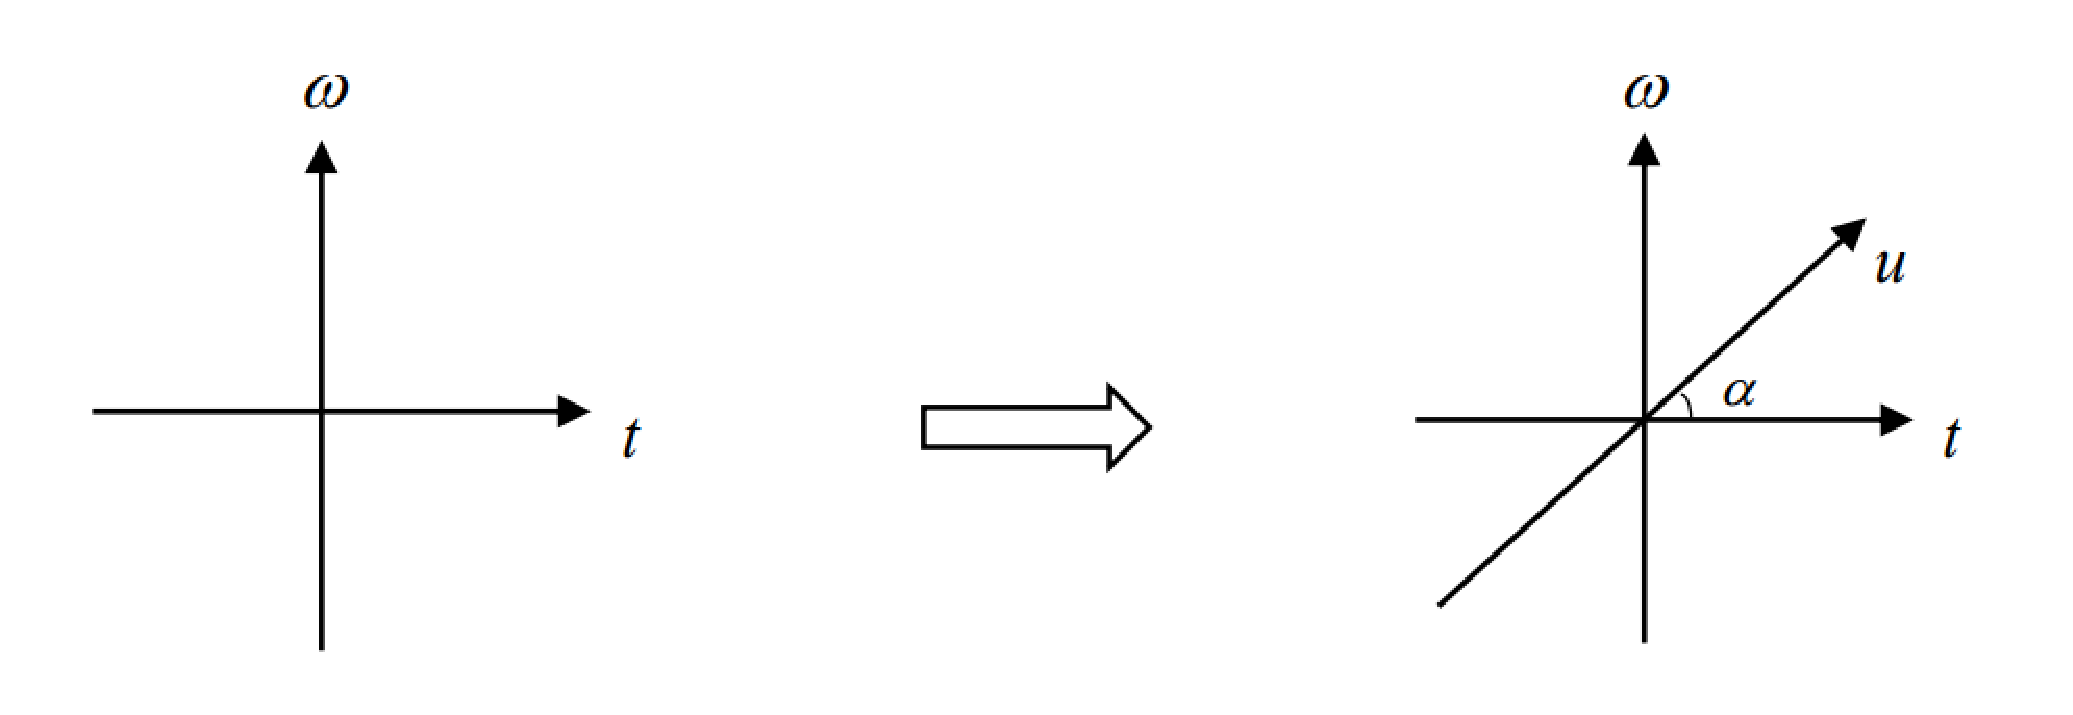
\includegraphics[width = 0.7\textwidth]{figure2_1.eps}
\caption{时频平面旋转示意图}\vspace{-1em}\label{shipinxuanzhuan}
\end{figure}

分数傅里叶变换有着多种定义方式,大致可以分为两大类:经典类分数傅里叶变换(CFRFT)和加权类分数傅里叶变换(WFRFT)。这里仅介绍加权类分数傅里叶变换。加权分数傅里叶变换是~C.Shih~利用态函数叠加方法提出的一种新的分数傅里叶变换定义。基本思想是利用经典傅里叶变换整数幂运算的~4~周期性,将新的分数傅里叶变换定义成~4~个态函数的线性组合,组合系数则为分数傅里叶变换阶数的函数。对一个信号~$f(x)$~进行~0,1,2,3~次傅里叶变换的结果分别为~$f(x)$~,~$G(x)$~,~$f(-x)$~,~$G(-x)$~,这四个函数便是四项加权分数傅里叶变换(4-WFRFT)的基函数,WFRFT~的定义如下:
\begin{equation}
{\mathcal{F}^\alpha }\left[ {f\left( x \right)} \right] = {\omega _0}\left( \alpha  \right)f\left( x \right) + {\omega _1}\left( \alpha  \right)F\left( x \right) + {\omega _2}\left( \alpha  \right)f\left( { - x} \right) + {\omega _3}\left( \alpha  \right)F\left( { - x} \right)
\end{equation}
其中加权系数${\omega _l}(l = 0,1,2,3)$的定义如下:
\begin{equation}\label{jiaquanxishu}
{\omega _l}(\alpha ) = \cos \left[ {\frac{{(\alpha  - l)\pi }}{4}} \right]\cos \left[ {\frac{{2(\alpha  - l)\pi }}{4}} \right]\exp \left[ {\frac{{3(\alpha  - l)\pi j}}{4}} \right]\;\;\;\;\;(l = 0,1,2,3)
\end{equation}
决定加权系数的变换阶数~$\alpha$~一样以~4~为周期,在~$[0,4]$~区间内变换,图~\ref{xishubianhua}~表明当变换阶数~$\alpha$~变化时,加权系数幅值的变化情况。
\begin{figure}[htbp]
\centering
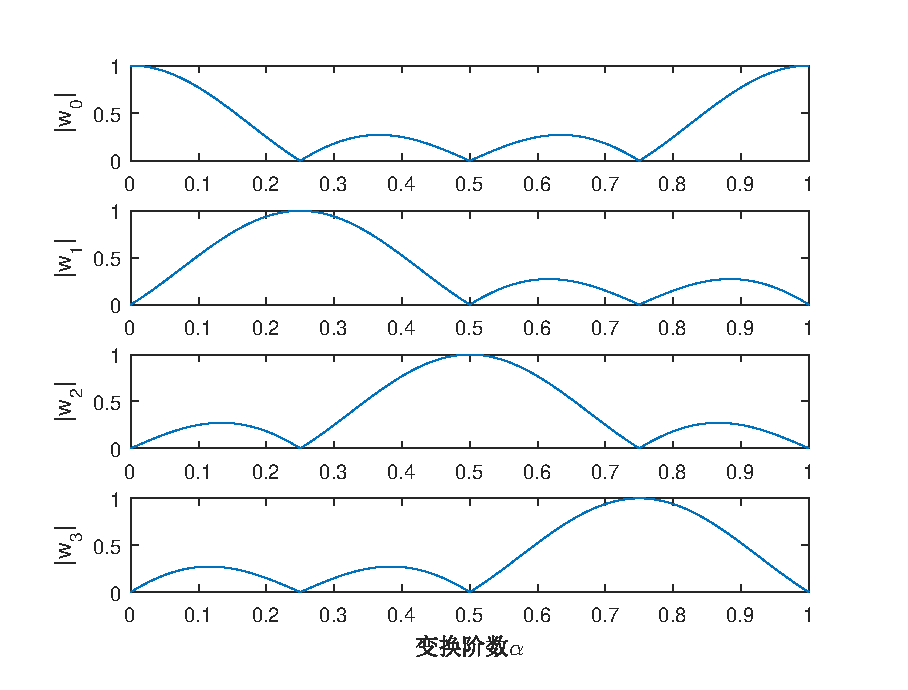
\includegraphics[width = 0.8\textwidth]{figure2_2.eps}
\caption{加权系数的模随变换阶数~$\alpha$~的变化}\vspace{-1em}\label{xishubianhua}
\end{figure}

不难从图中看出随着变换阶数的变化,在~4-WFRFT~后的函数中,原函数与经过傅里叶变换后函数所占比重在发生变化,$\alpha$~逐渐靠近~1~和~3~时,傅里叶变换后函数所占比重在不断增大,$\alpha$~逐渐靠近~0~和~2~时,原函数所占比重在不断增大。

这种加权形式定义的~WFRFT~实现的过程比经典~FRFT~简单,并且也满足一些~FRFT~的性质:
\begin{itemize}
\item 连续性:$\left\{ {{\mathcal{F}^\alpha }:{L^2}\left( R \right) \to {L^2}\left( R \right)} \right\}$~,且~$\alpha$~为连续可变的实数;
\item 边界性:当~$\alpha$~取值为整数时,WFRFT~退变为经典傅里叶变换;
\item 旋转相加性:${\mathcal{F}^\alpha }\left\{ {{\mathcal{F}^\beta }\left[ {f\left( x \right)} \right]} \right\} = {\mathcal{F}^{\alpha  + \beta }}\left[ {f\left( x \right)} \right]$~;
\item 酉性:${\left( {{\mathcal{F}^\alpha }} \right)^{ - 1}} = {\left( {{\mathcal{F}^\alpha }} \right)^H}~$。
\end{itemize}

可以看出,经典~WFRFT~的信号表达形式是一种表达时间与频率的连续函数,然而在实际系统中,这种信号无法产生,因此较大程度限制了其在通信系统中的应用。若想将~WFRFT~应用在通信系统中有必要对其进行离散化,传统离散傅里叶变换~DFT~也同样以~4~为周期,而任意一个具有周期性的算子,均可以通过态函数加权的方式进行分数化,因此这里直接利用~DFT~给出了任意复数序列的~4-WFRFT~。

首先定义一个长度为~$N$~的复数序列~${X_0}$~,${X_1}$~、${X_2}$~、${X_3}$~分别为此序列进行~1~,2~,3~次~DFT~的结果,其能量归一化的~DFT~形式如下
\begin{equation}
\left\{ \begin{array}{l}
{X_1}\left( k \right) = \frac{1}{{\sqrt N }}\sum\limits_{n = 0}^{N - 1} {{X_0}\left( n \right){e^{ - j\frac{{2\pi }}{N}kn}}} \\
{X_0}\left( n \right) = \frac{1}{{\sqrt N }}\sum\limits_{n = 0}^{N - 1} {{X_1}\left( k \right){e^{j\frac{{2\pi }}{N}kn}}}
\end{array} \right.
\end{equation}

参照~WFRFT~的定义公式,序列的离散~WFRFT~定义如下:
\begin{equation}
{S_0} = {\mathcal{F}^\alpha }\left[ {{X_0}} \right] = {\omega _0}\left( \alpha  \right){X_0} + {\omega _1}\left( \alpha  \right){X_1} + {\omega _2}\left( \alpha  \right){X_2} + {\omega _3}\left( \alpha  \right){X_3}
\end{equation}

采用矩阵的形式表示如下
\begin{equation}
  \begin{array}{l}
  {\bf{S}} = \left[ \begin{array}{l}
  {S_0}\\
  {S_1}\\
  {S_2}\\
  {S_3}
  \end{array} \right] = {{\bf{W}}_\alpha }{\bf{X}} = \left[ {\begin{array}{*{20}{c}}
  {{\omega _0}}&{{\omega _1}}&{{\omega _2}}&{{\omega _3}}\\
  {{\omega _3}}&{{\omega _0}}&{{\omega _1}}&{{\omega _2}}\\
  {{\omega _2}}&{{\omega _3}}&{{\omega _0}}&{{\omega _1}}\\
  {{\omega _1}}&{{\omega _2}}&{{\omega _3}}&{{\omega _0}}
  \end{array}} \right]\left[ \begin{array}{l}
  {X_0}\\
  {X_1}\\
  {X_2}\\
  {X_3}
  \end{array} \right]\\
  \;\;\;\;\;\;\;\;\;\;\;\;\;\;\;\;\;\;\;\;\;\; = \left[ {\begin{array}{*{20}{c}}
  {{\omega _0}{X_0} + {\omega _1}{X_1} + {\omega _2}{X_2} + {\omega _3}{X_3}}\\
  {{\omega _3}{X_0} + {\omega _0}{X_1} + {\omega _1}{X_2} + {\omega _2}{X_3}}\\
  {{\omega _2}{X_0} + {\omega _3}{X_1} + {\omega _0}{X_2} + {\omega _1}{X_3}}\\
  {{\omega _1}{X_0} + {\omega _2}{X_1} + {\omega _3}{X_2} + {\omega _0}{X_3}}
  \end{array}} \right]
  \end{array}
\end{equation}
其中,${S_1}$~,${S_2}$~,${S_3}$~分别是序列~${S_0}$~的~1~,2~,3~次~DFT~。可以看出~${S_0}$~,${S_1}$~,${S_2}$~,${S_3}$~分别是~${X_0}$~,${X_1}$~,${X_2}$~,${X_3}$~的~$\alpha$~阶~WFRFT~变换且满足如下关系:
\begin{equation}
{S_3} = \mathcal{F}[{S_2}] = {\mathcal{F}^2}[{S_1}] = {\mathcal{F}^3}[{S_0}]
\end{equation}

通过上面给出的定义形式,可以看出~WFRFT~可以对输入的任意复数序列进行变换并通过相应阶数的逆变换还原原始输入序列。可以直接应用于通信系统中。需要注意的,离散化~WFRFT~的变换结果并不等同于对传统的~WFRFT~进行采样,这点与傅里叶变换与~DFT~的关系不同,原因在于若对经典~WFRFT~采样,其时域和频域的量纲不统一。

%%%%%%%%%%%%%%%%%%%%%%%%%%%%%%%%%%%%%%%%%%%%%%%%%%%%%%%%%%%%%%
\subsection{基于~4-WFRFT~的变换域通信系统}

对于四项加权形式定义的~FRFT~,在计算某一信号的~4-WFRFT~时,由于~4~个加权项的特殊性,实际上就是对信号的时域信息和频域信息进行加权相加,因此它的计算复杂度要小于经典定义类型的~FRFT~,因其是通过~DFT~定义的,在计算中可以直接利用快速傅里叶算法~FFT~计算,计算量与~FFT~相当,也因此更容易在工程中实现。

~4-WFRFT~模块的物理实现过程如图~\ref{jiaquanshixianguocheng}~:
\begin{figure}[htbp]
\centering
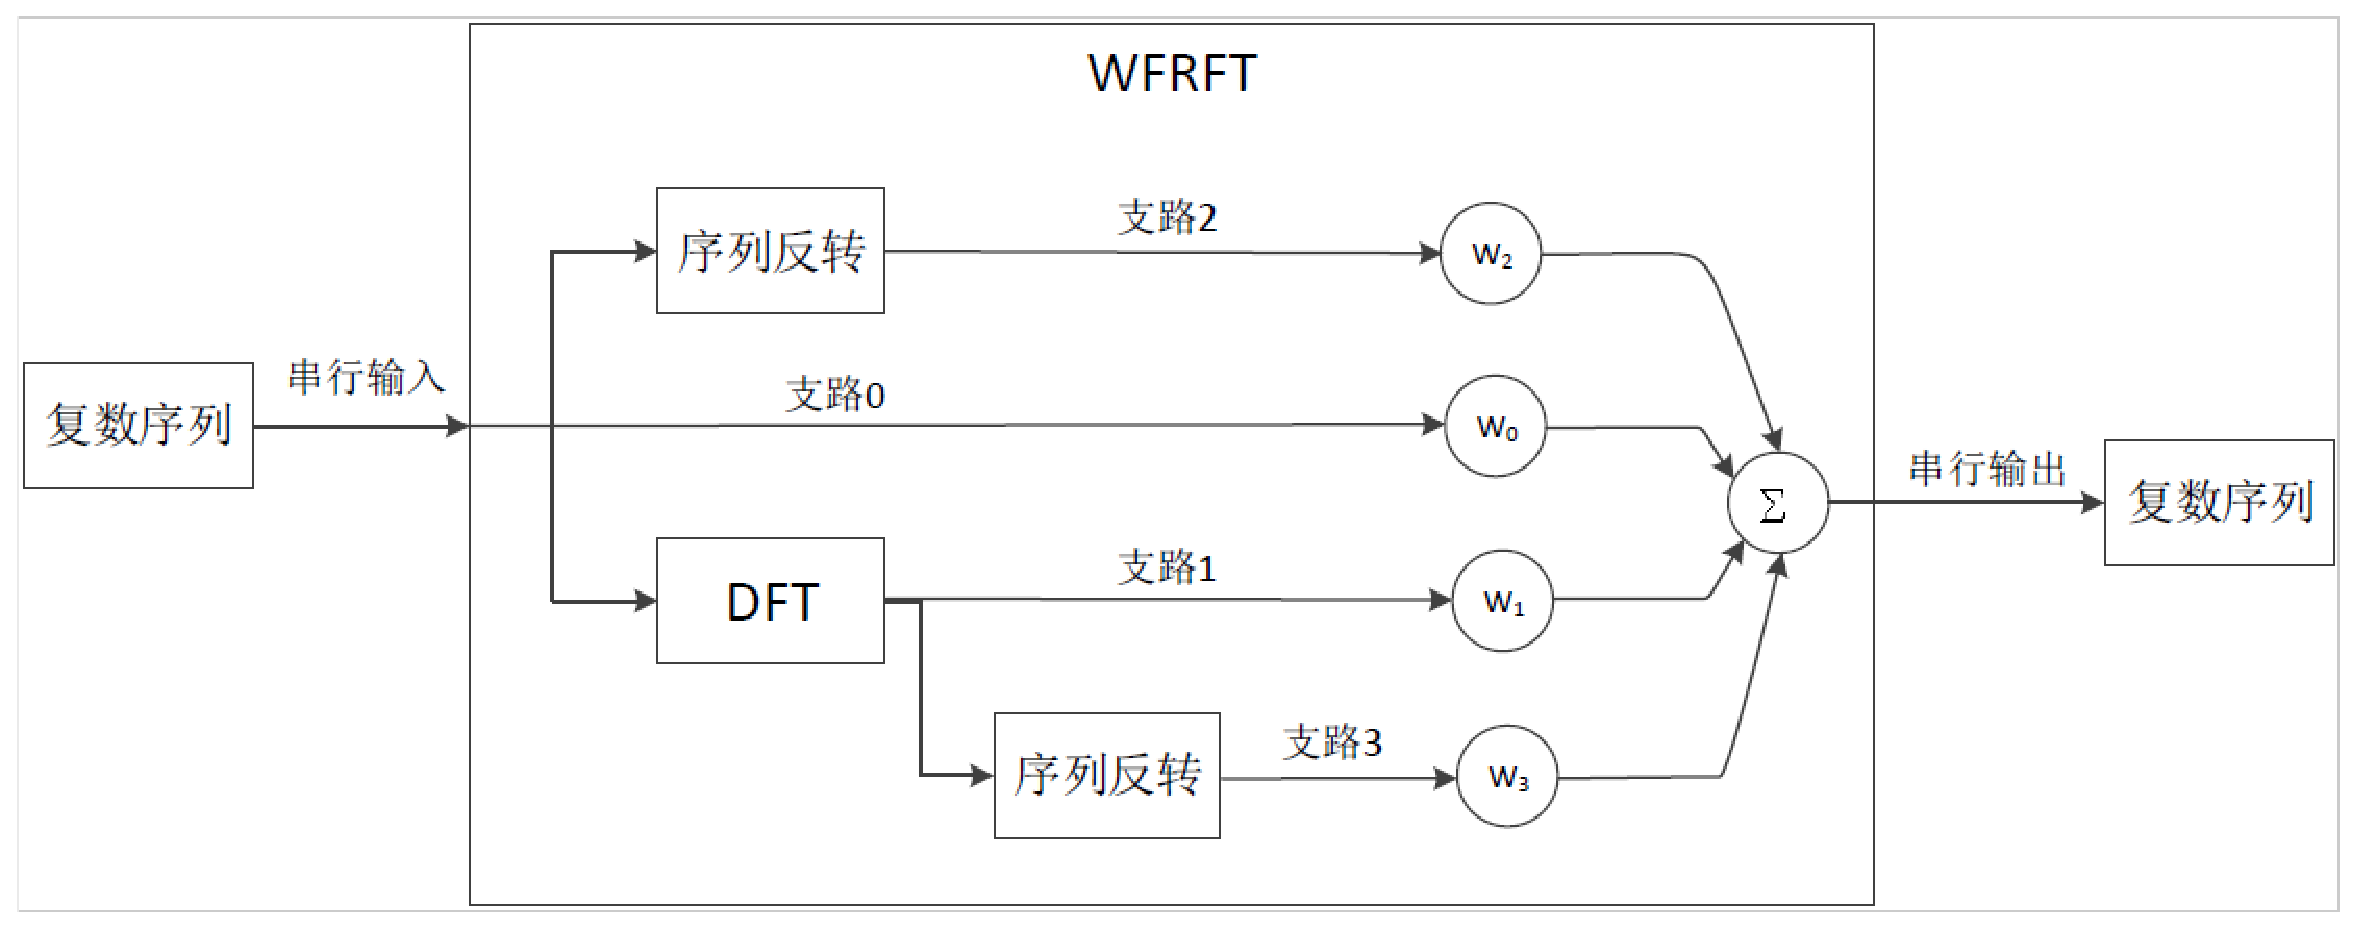
\includegraphics[width = 0.8\textwidth]{figure2_4.eps}
\caption{4-WFRFT~物理实现过程}\vspace{-1em}\label{jiaquanshixianguocheng}
\end{figure}
长度为~$N$~的复数序列~$X_0$~为原始需调制信号,分四路进行加权求和,其中两路为原始时域信号与其反转后的信号,另外两路信号为原始序列经~DFT~的结果与其反转,在实现过程中当~$N$~为~2~的整数次幂时可以直接用~FFT~模块代替~DFT~,即完成一次~4-WFRFT~变换仅需一次~DFT~和两次信号反转,计算量与实际系统中实现的复杂程度与~FFT~相近。容易在通信系统中实现。其变换过程数学模型如下:
\begin{equation}\label{WFRFTgongshi}
\begin{split}
{S_0}(n) = {w_0} \cdot {X_0}(n) + {w_1} \cdot \frac{1}{{\sqrt N }}\sum\limits_{k = 0}^{N - 1} {{X_0}(k){e^{ - j\frac{{2\pi }}{N}kn}}}\\
 +  {w_2} \cdot {X_0}( - n) + {w_3} \cdot \frac{1}{{\sqrt N }}\sum\limits_{k = 0}^{N - 1} {{X_0}(k){e^{j\frac{{2\pi }}{N}kn}}}
\end{split}
\end{equation}

对比~OFDM~系统和单载波频域均衡系统的实现结构不难看出:支路~1~,3~均经过~DFT~处理后进行加权,对应了~OFDM~信号的并行传输过程;而另外两支路没有~DFT~模块仅是一次反转,没有其他处理操作,实际上是简单的单载波串行传输的过程。实际上,由于~4-WFRFT~定义形式的特殊性,对信号进行~4-WFRFT~的过程中的时域频域信息与现有通信系统中对信号进行单载波和多载波调制的表述形式相一致。可以看成~4-WFRFT~是将单载波系统与多载波系统融合起来,实现的混合载波调制。并且~4-WFRFT~输出信号的时频特征与其调制阶数~$\alpha$~有直接关系,改变参数~$\alpha$~可以实现单载波调制与多载波调制之间的转换,使用于现有的通信发射、接受系统,不需要额外开销。WFRFT~通信系统较之于传统通信系统由于加权阶数的引入,可以更加灵活的应对某些特定信道条件,可以通过搜寻最优化的变换阶数~$\alpha$~来使系统整体性能最优化。

基于~WFRFT~在数字通信中的物理意义,文献[]的作者给出了混合载波通信系统模型如图~\ref{xitongjiegou}~:
\begin{figure}[htbp]
\centering
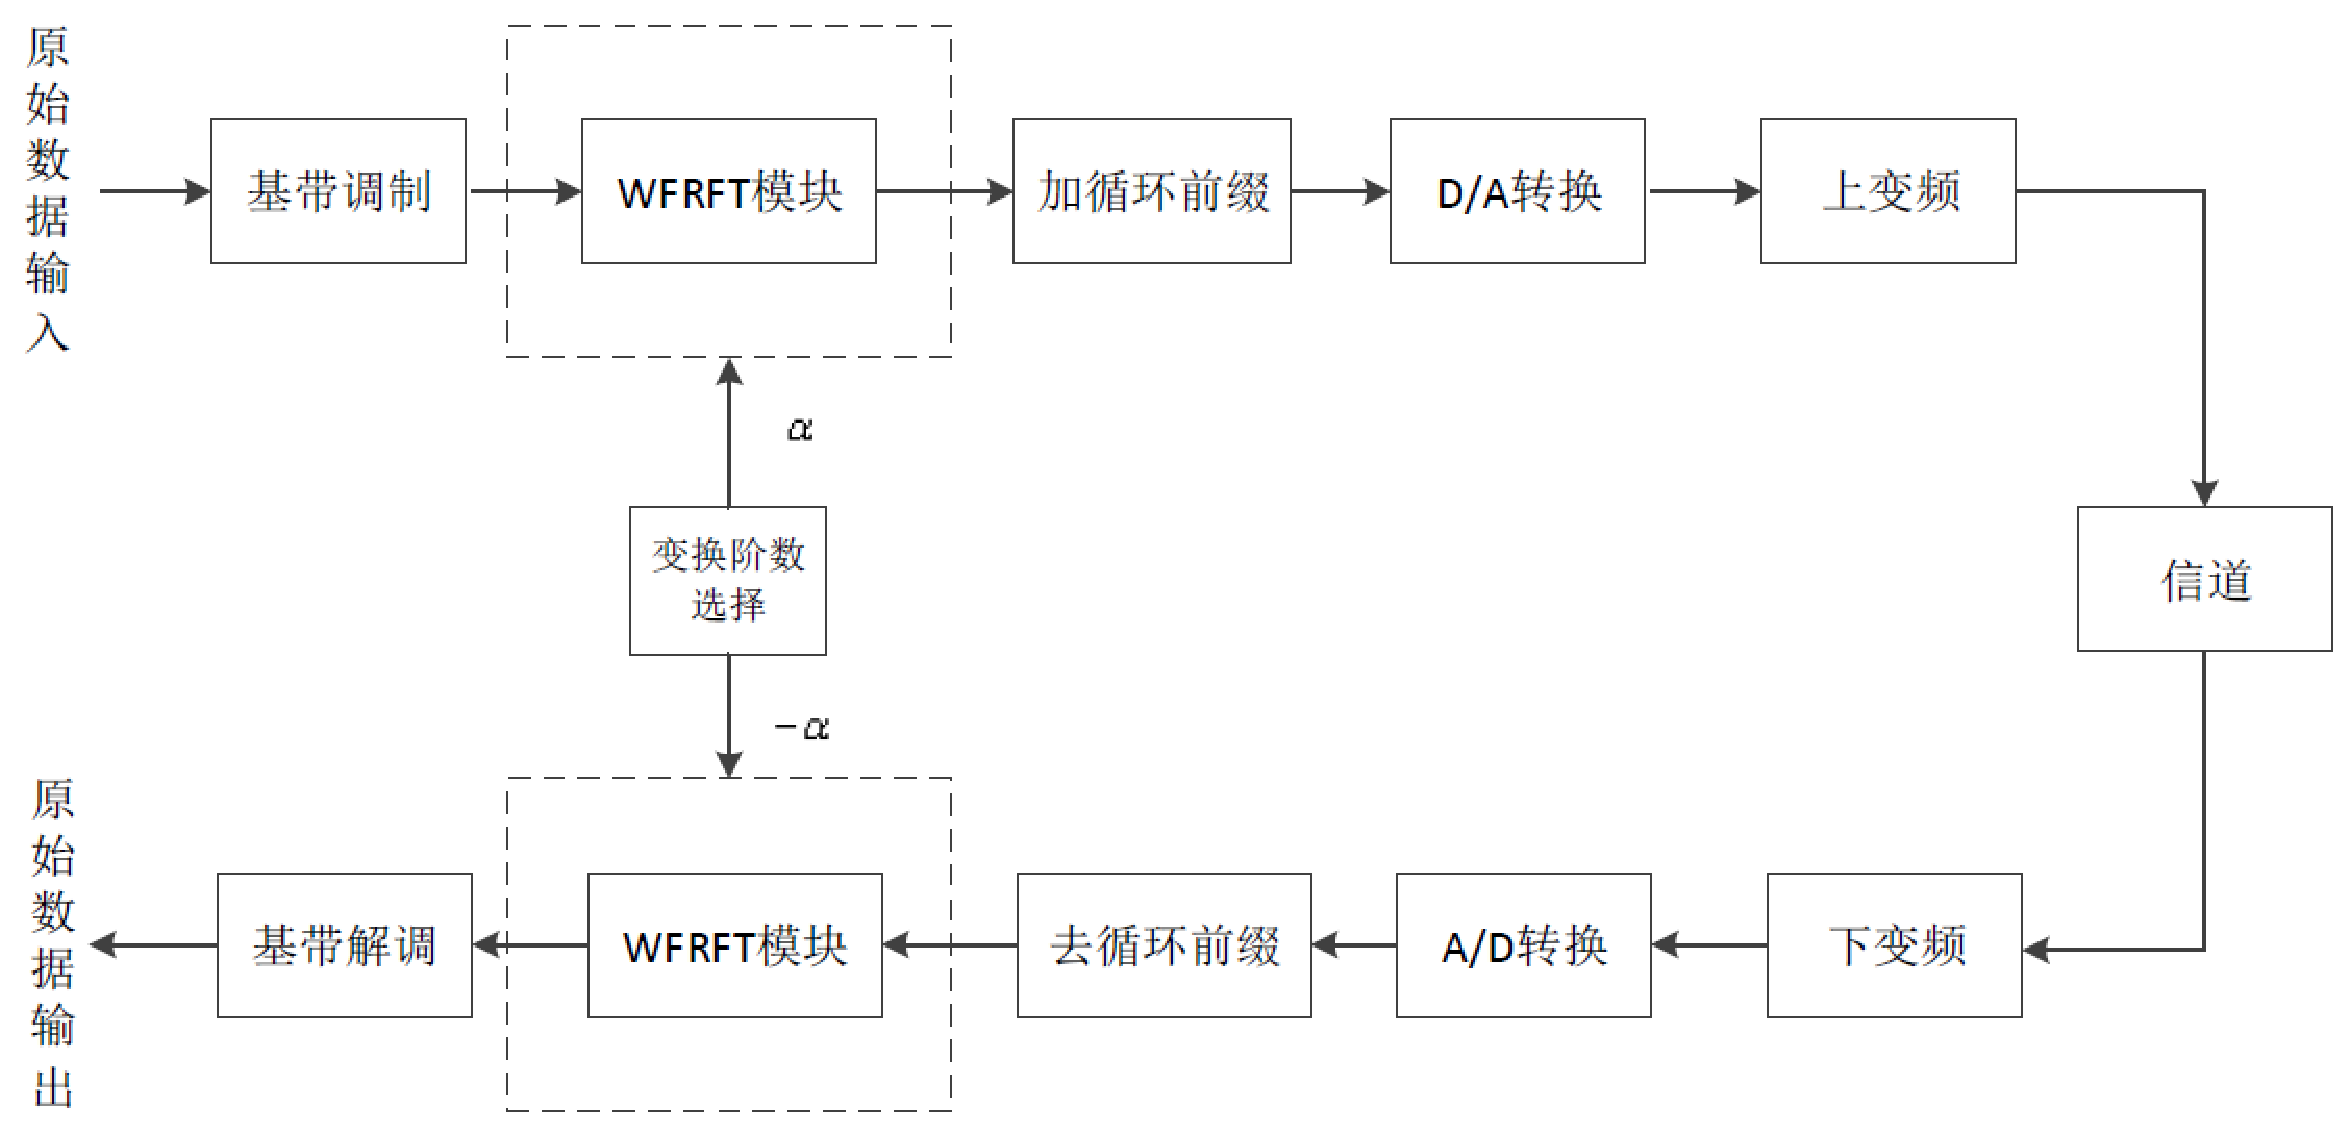
\includegraphics[width = 0.8\textwidth]{figure2_3.eps}
\caption{基于~4-WFRFT~通信系统结构}\vspace{-1em}\label{xitongjiegou}
\end{figure}

从图中可以看出,混合载波通信系统与~OFDM~系统相似,该通信系统模型可以在基于块传输方式的单载波和~OFDM~系统之间实现平滑过渡:通过阶数~$\alpha$~进行转换,当~$\alpha$~为非整数时,系统对应为单载波与多载波的混合形式。这一方面可以作为沟通传统单载波、多载波体制的桥梁;另一方面,在很多复杂、多变的环境或条件约束下,混合载波通信系统可能具有较传统载波体制更灵活的应对方式和更好的性能表现。

从上面的分析得到,~4-WFRFT~对信号的处理过程实际上包含了单载波与多载波的实现过程,所以,~4-WFRFT~变换后的信号特征也与传统调制下的信号有所不同。根据式~(\ref{WFRFTgongshi})~给出的~4-WFRFT~数学表达定义可以看出,~4-WFRFT~的输出信号形式不仅仅与输入信号的信息有关,在很大程度上由加权系数来决定变换后信号中所含时频信息的比重,加权系数又由变换阶数~$\alpha$~决定,当~$\alpha$~变化时引起各个加权信号的幅值伸缩与相位旋转,从而决定了~4-WFRFT~输出信号的不同。

图~\ref{xingzuotu}~给出了~QPSK~信号分别经过变换阶数为~0~,0.1~,0.25~,1~的~4-WFRFT~变换处理后的星座图,
\begin{figure}[htbp]
\centering
\subfigure{\label{xingzuo1}}\addtocounter{subfigure}{-2}
\subfigure{\subfigure[~$\alpha$~= 0]{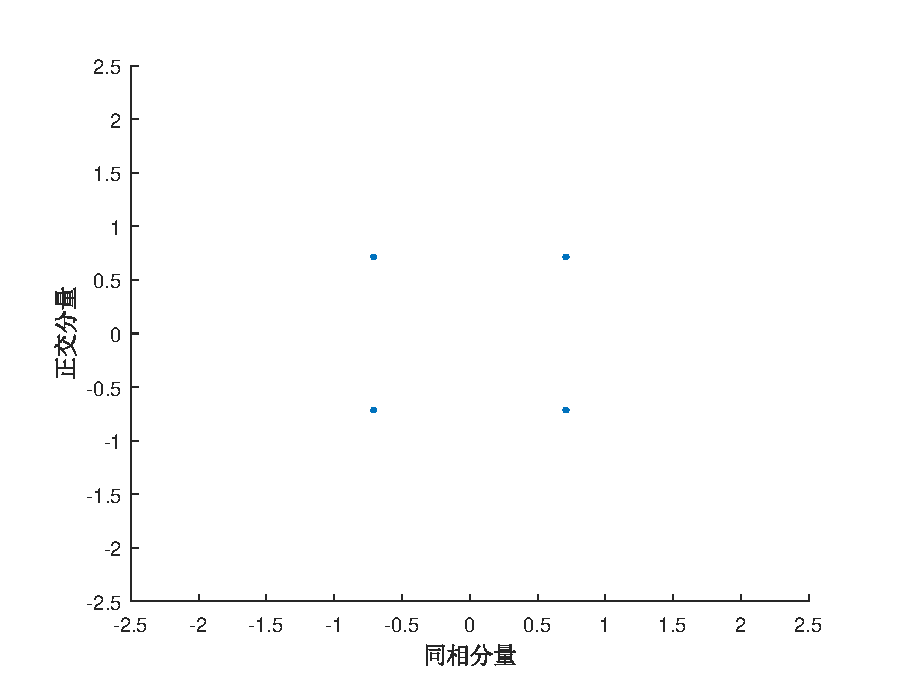
\includegraphics[width=0.36\textwidth]{xingzuo0.eps}}}
\subfigure{\label{xingzuo2}}\addtocounter{subfigure}{-2}
\subfigure{\subfigure[~$\alpha$~= 0.1]{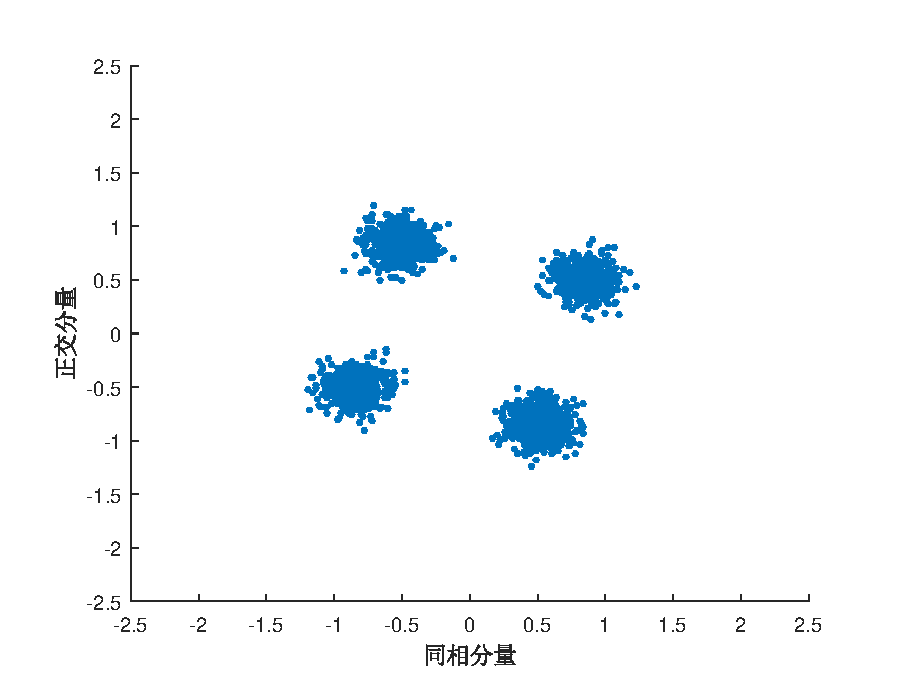
\includegraphics[width=0.36\textwidth]{xingzuo01.eps}}}
\subfigure{\label{xingzuo3}}\addtocounter{subfigure}{-2}
\subfigure{\subfigure[~$\alpha$~= 0.25]{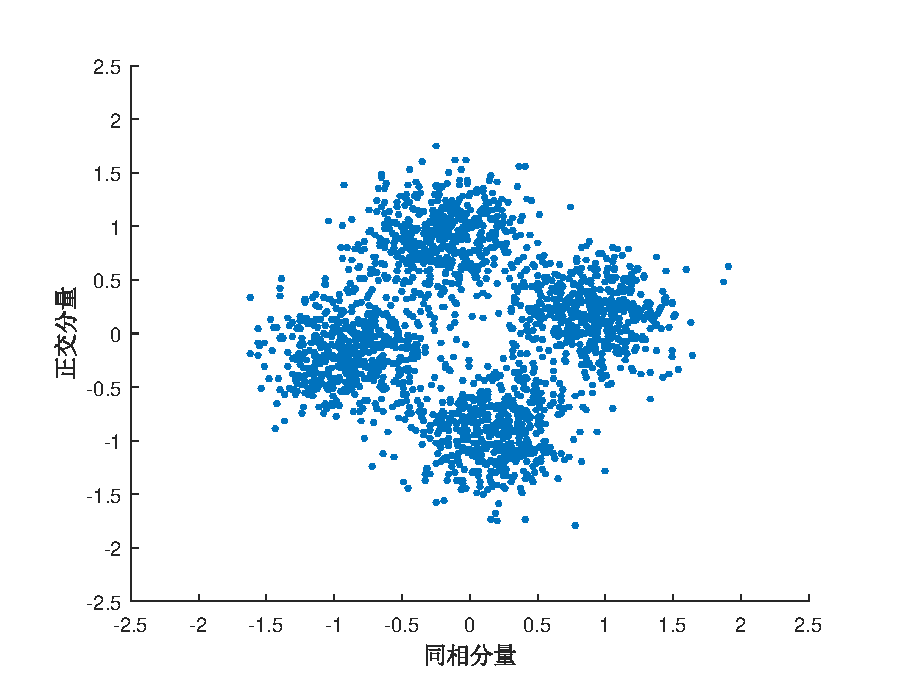
\includegraphics[width=0.36\textwidth]{xingzuo025.eps}}}
\subfigure{\label{xingzuo4}}\addtocounter{subfigure}{-2}
\subfigure{\subfigure[~$\alpha$~= 1]{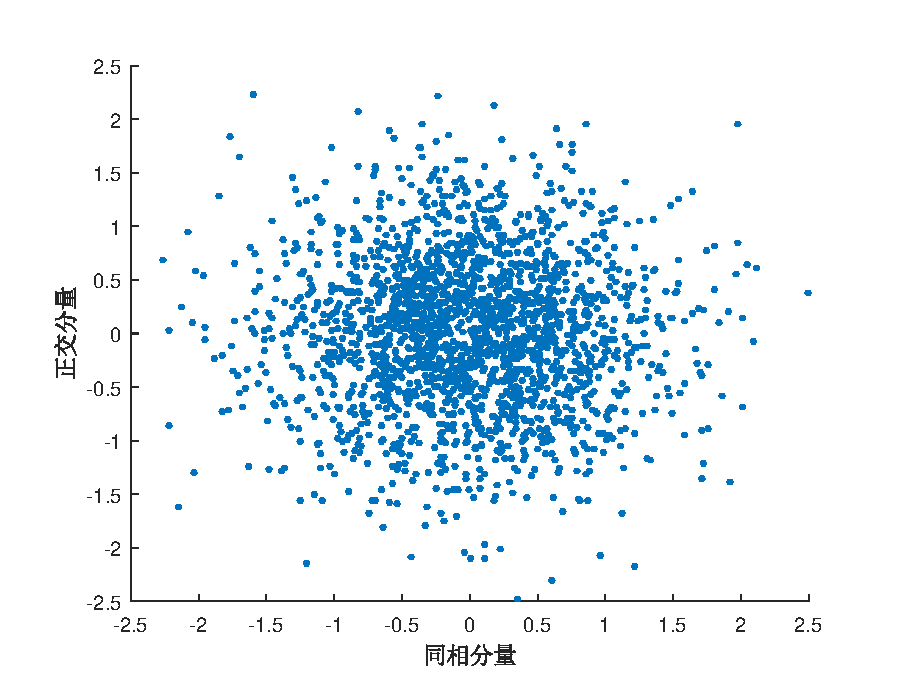
\includegraphics[width=0.38\textwidth]{xingzuo1.eps}}}
\caption{~4-WFRFT~变换后信号星座图}\label{xingzuotu}\vspace{-1em}
\end{figure}
可以看出随着~$\alpha$~的增大,原本重叠在一起的星座点逐渐旋转并散开,随着~$\alpha$~进一步增大,星座点的边界逐渐模糊,信号所含频域成分逐渐增加,最终当~$\alpha$~增大到~1~时,所有信号点完全混叠在一起,无法区分,在复平面呈现出一种类高斯的分布,在接收端只有通过与之对应的~$-\alpha$~阶反变换才能够将信号正确解调。通过信号星座图的描绘,展现了~WFRFT~信号灵活多变的特点。单参数~WFRFT~信号的星座图会随着阶数的改变而呈现发散、 旋转、 汇聚等变化, 星座点分布呈现类高斯特性。WFRFT~的这种信号形式比传统比传统单载波和多载波信号具有更均匀的时频能量分布。这一分布特性有利于信号在复杂多变的场景中,以及时频域同时存在干扰的信道下保持性能鲁棒性。

% !Mode:: "TeX:UTF-8"

\section{已完成的研究工作}
\subsection{同步偏差对混合载波通信系统的影响}

混合载波通信系统发射信号会同时包含单载波分量和多载波分量。也就是说变换域通信系统的信号特征同时继承了单载波通信系统和多载波通信系统的信号特点,然而也同样因此不仅继承了两种通信系统的优点,也保留了缺点。我们知道,单载波系统由于其在时域中进行符号判决,因而对定时偏差非常敏感,而多载波系统由于传输性能是仪子载波间的正交性为基础的,很小的频率偏差就会破坏正交性,从而极大影响系统性能,因此对于混合载波通信系统而言,精准的定时同步和频率偏差矫正非常重要。

在实际通信系统中,引起同步误差最主要的原因是收发双方晶振时钟不一致,从而导致的在接收端的采样时刻的误差和收发双方的载波频率不同步, 根据前面已经分析了混合载波的通信系统模型,图~\ref{jiaquanshixianguocheng}~给出存在同步偏差的信道模型:
\begin{figure}[htbp]
\centering
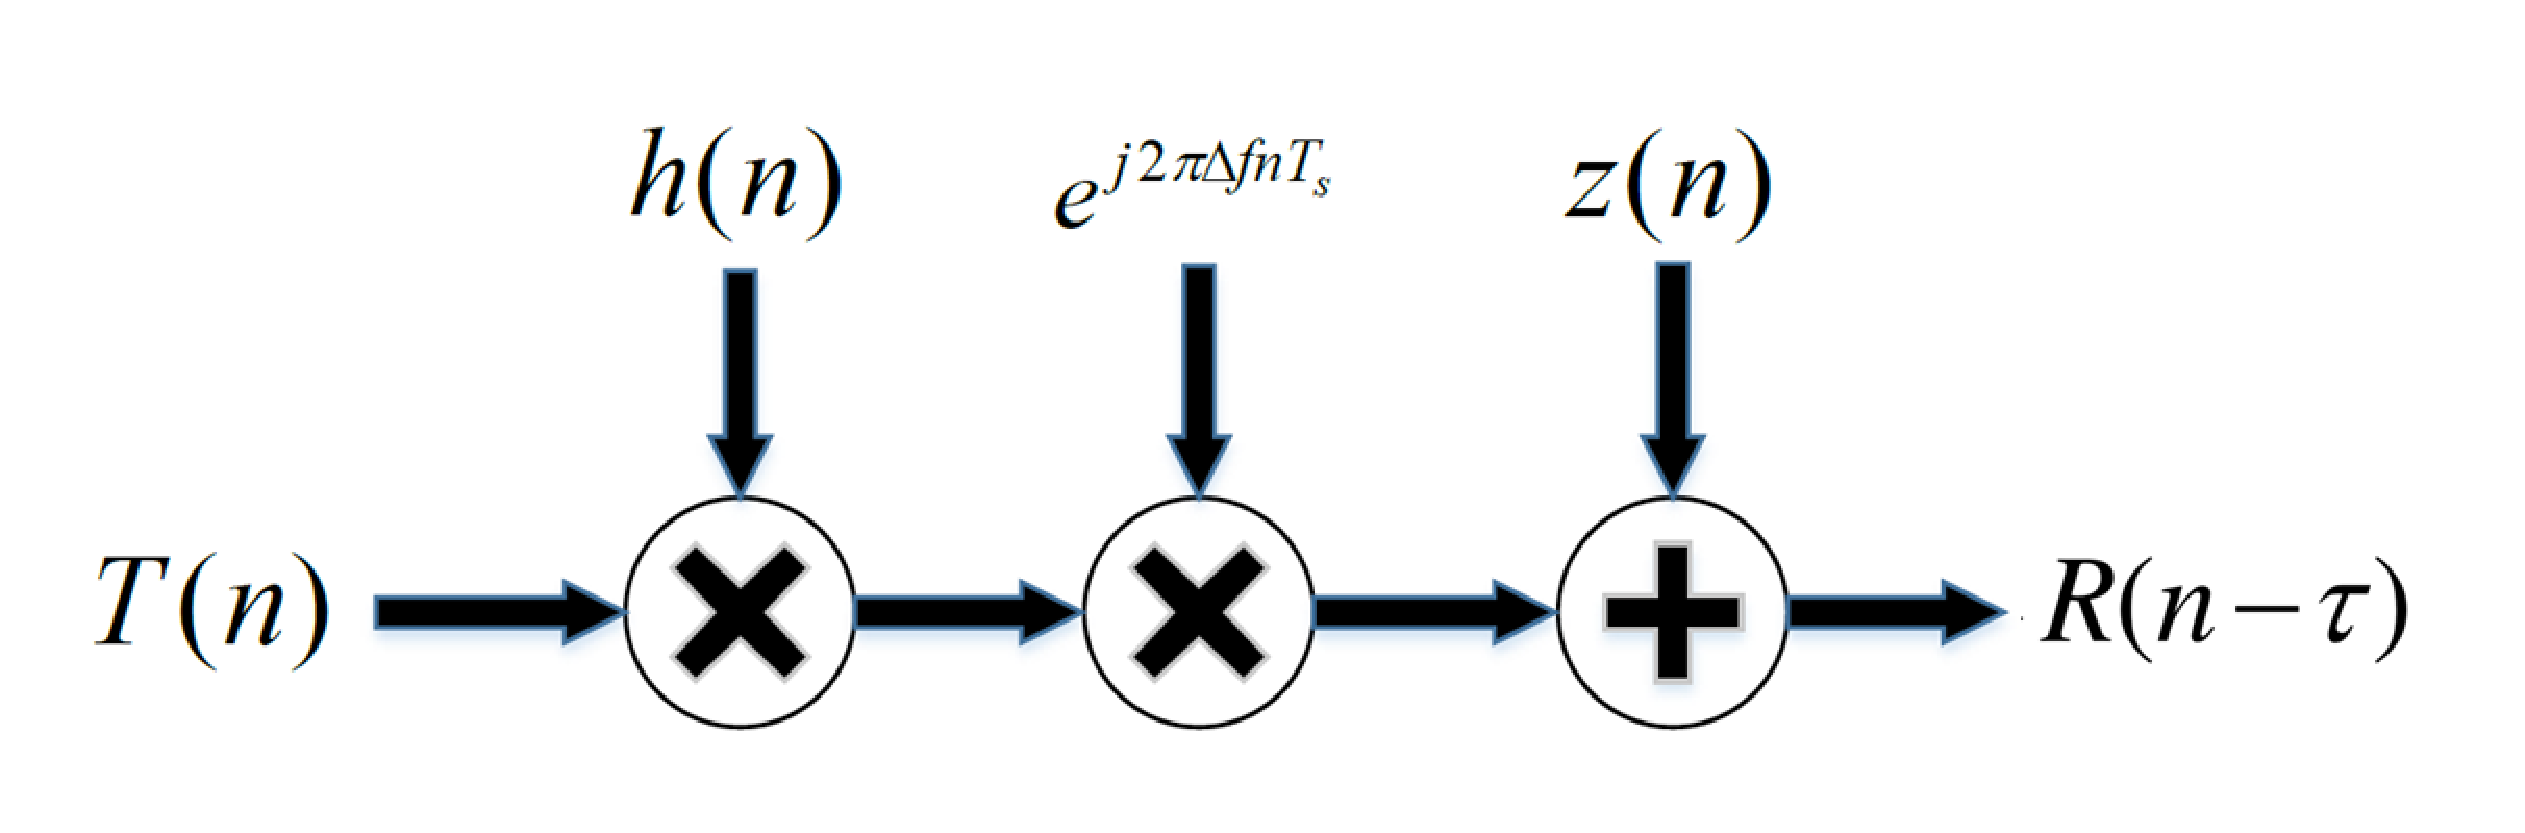
\includegraphics[width = 0.6\textwidth]{figure4_1.eps}
\caption{信道模型}\vspace{-1em}\label{xindaomoxing}
\end{figure}
其中~$T(n)$~为混合载波通信系统发射端发送到信道中的时域信号,即基带调制后的信号~$X(n)$~进行~$\alpha$~阶~4-WFRFT~变换的结果,$h(n)$~为信道的冲激相应,$R(n)$~为发射信号~$T(n)$~经过信道并且在接收端下变频后接收到的信号。为了后续理论分析与讨论的简便,这里假设信道是平缓的即~$h(n)=1$,信号仅受到频偏与加性高斯白噪声~$z(n)$~的影响,并在接受端存在一定时延。这里简化系统发射接收时上下变频的过程,将发射端与接收端由于晶振偏差产生的本地载波频率偏差引入到信道中,其中~$\Delta f$~表示发射与接收端本地载波频差,$T_s$~表示发送端基带数据采样间隔。

根据第~2~章的WFRFT理论,设变换前基带信号为~$X(n)$~,
%则发射信号如公式~(\ref{fashexinhao})~所示
%\begin{equation}\label{fashexinhao}
%\begin{split}
%T(n) = w_0^\alpha X(n) + w_1^\alpha  \cdot \frac{1}{{\sqrt N }}\sum\limits_{k = 0}^{N - 1} {X(k){e^{ - j\frac{{2\pi }}{N}kn}}} \\
%  + w_2^\alpha X( - n) + w_3^\alpha  \cdot \frac{1}{{\sqrt N }}\sum\limits_{k = 0}^{N - 1} {X(k){e^{j\frac{{2\pi }}{N}kn}}}
%\end{split}
%\end{equation}
这里为了讨论方便,将分别推导采样时间偏差和频率偏差对混合载波通信系统影响。首先讨论当仅存在定时偏差的情况,混合载波定时同步的示意图如下:
\begin{figure}[htbp]
\centering
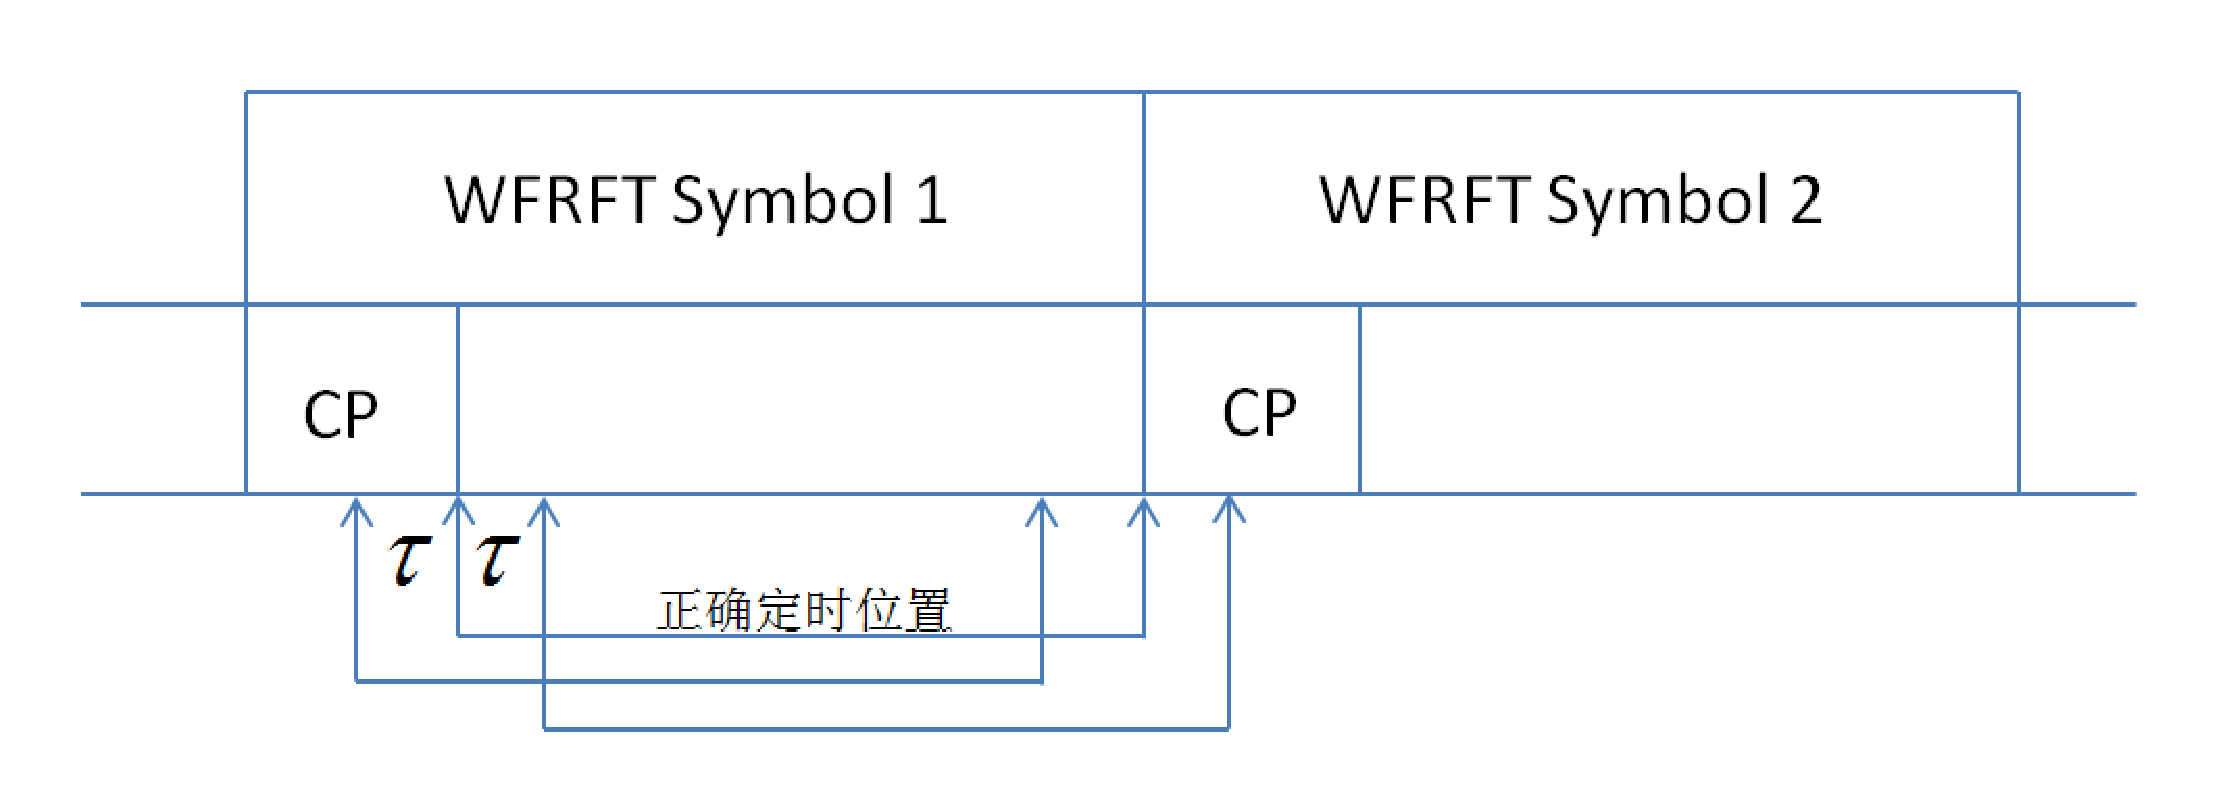
\includegraphics[width = 0.8\textwidth]{figure4_2.eps}
\caption{定时同步示意图}\vspace{-1em}\label{dingshitongbuweizhi}
\end{figure}

接收端的基带信号表现形式如下:
\begin{equation}
R(n-\tau) = T(n-\tau) + z(n-\tau)
\end{equation}

当接收端时间同步不精确,定时同步的起点位于循环前缀内部时,
\begin{align}\label{huajianjieguo}
\tilde X_i(n) &= {\mathcal{F}^\alpha }\left ( R_i\left ( n-\tau \right ) \right ) \\
&= w_0^{- \alpha }R_i(n-\tau) + w_1^{- \alpha }{{\mathcal{F}^1}\left ( R_i\left ( n-\tau \right ) \right )}
+ w_2^{- \alpha }{{\mathcal{F}^2}\left ( R_i\left ( n-\tau \right ) \right )}
+ w_3^{- \ }{{\mathcal{F}^3}\left ( R_i\left ( n-\tau \right ) \right )} \\
&= \underbrace {w_0^{- \alpha }R_i(n-\tau) + w_2^{- \alpha }R_i(\tau -n)}_{ISI} + w_1^{- \alpha }{{\mathcal{F}}\left ( R_i\left ( n \right ) \right )} {e^{-j2\pi \frac{{\varepsilon n}}{N}}} + w_3^{- \alpha }{{\mathcal{F}}\left ( R_i\left ( -n \right ) \right )} {e^{-j2\pi \frac{{\varepsilon n}}{N}}}
\end{align}

其中~$R_i(n)$~代表接受到的第i个WFRFT符号的第~$n$~个采样点,从式中可以看出,由于单载波分量的存在,定时同步误差将引入符号间干扰(ISI),而第二与第四分量虽然会产生一个相位因子,但并未产生干扰。而若当定时同步起点位于循环前缀外时,此时这一符号的采样信息会包含下一符号的信息,不仅引入了符号间干扰,同时也会在多载波分量间引入载波间干扰~ICI,这种情况下将严重影响通信性能,应是极力避免的,在此便不详细推导了。
\begin{figure}[htbp]
\centering
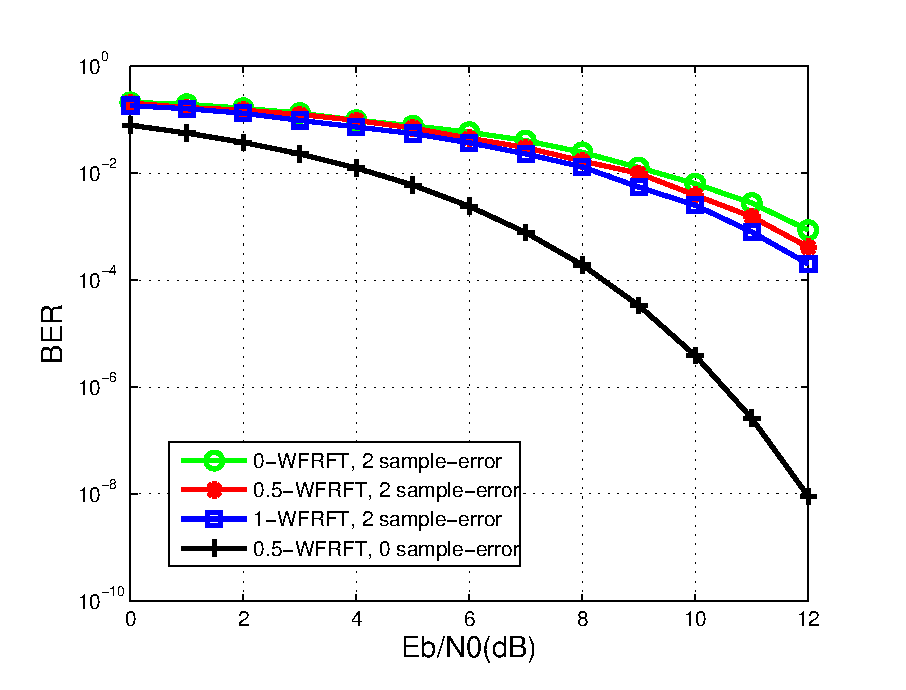
\includegraphics[width = 0.8\textwidth]{plot_ber_at_time_error.eps}
\caption{不同调制阶数下HC系统在2个定时误差下误码性能比较}\vspace{-1em}\label{plot_ber_at_time_error}
\end{figure}
图~\ref{plot_ber_at_time_error}~给出了~AWGN~信道下混合载波通信系统当在非最佳采样点下误码性能的比较,仿真参数选择一个~WFRFT~符号载波数为2048,数据符号所占载波数为1200,采用16倍上采样,收发双方均采用升余弦滚降滤波器进行铝箔,在接受端存在~2~个采样点的误差进行解调下,当调制阶数~1~时,此时混合载波通信系统只包含多载波通信过程,此时系统抗定时误差性能最强。当调制阶数~0~时,混合载波通信系统只包含单载波成分,其性能受定时误差影响较大大。当调制阶数介于~0~到~1~之间时,此时混合载波通信系统同时包含有单载波成分和多载波成分,且阶数越小,包含的单载波成分也越多,此时受定时采样误差影响也越大。从图中也可以看出,虽然仅仅有2个采样点误差,但与最佳采样点的系统性能相差巨大,故定时同步对系统性能的保证十分关键。

另一方面,当混合载波通信系统中存在频偏影响时,发射信号受到频偏的影响在接收端的基带信号表示形式如为~$R(n) = T(n){e^{j2\pi \Delta f(n){T_s}}} + z(n)$~。接收端的解调过程需对接收信号进行~$-\alpha$~阶~4-WFRFT~变换以恢复原始信号~$X(n)$~,将接收信号代入解调公式可以得出解调结果数学表达式如公式~(\ref{jietiaojieguo})~所示:
\begin{eqnarray}\label{jietiaojieguo}
%\begin{array}{l
\tilde X(n) &=& (w_0^{ - \alpha }w_0^\alpha  + w_2^{ - \alpha }w_2^\alpha )X(n){e^{j2\pi \frac{{\varepsilon n}}{N}}} \nonumber \\
&+& {\rm{ }}w_1^{ - \alpha }w_3^\alpha \frac{1}{N}\sum\limits_{k = 0}^{N - 1} {\sum\limits_{m = 0}^{N - 1} {X(m){e^{j2\pi \frac{{mk}}{N}}}{e^{j2\pi \frac{{\varepsilon k}}{N}}}{e^{ - j2\pi \frac{{kn}}{N}}}} } \nonumber \\
&+& {\rm{ }}w_3^{ - \alpha }w_1^\alpha \frac{1}{N}\sum\limits_{k = 0}^{N - 1} {\sum\limits_{m = 0}^{N - 1} {X(m){e^{ - j2\pi \frac{{mk}}{N}}}{e^{j2\pi \frac{{\varepsilon k}}{N}}}{e^{j2\pi \frac{{kn}}{N}}}} } \nonumber \\
&+& {\rm{ (}}w_0^{ - \alpha }w_1^\alpha  + w_1^{ - \alpha }w_0^\alpha  + w_2^{ - \alpha }w_3^\alpha  + w_3^{ - \alpha }w_2^\alpha )\frac{1}{N}\sum\limits_{k = 0}^{N - 1} {\sum\limits_{m = 0}^{N - 1} {X(m){e^{ - j2\pi \frac{{mk}}{N}}}{e^{j2\pi \frac{{\varepsilon k}}{N}}}{e^{ - j2\pi \frac{{kn}}{N}}}} } \nonumber \\
&+& {\rm{ (}}w_3^{ - \alpha }w_1^\alpha  + w_1^{ - \alpha }w_3^\alpha  + w_1^{ - \alpha }w_2^\alpha  + w_2^{ - \alpha }w_1^\alpha )\frac{1}{N}\sum\limits_{k = 0}^{N - 1} {\sum\limits_{m = 0}^{N - 1} {X(m){e^{j2\pi \frac{{mk}}{N}}}{e^{j2\pi \frac{{\varepsilon k}}{N}}}{e^{j2\pi \frac{{kn}}{N}}}} } \nonumber \\
&+& Z(n)
%\end{array}
\end{eqnarray}
式中~$\varepsilon  = \Delta fN{T_s}$~表示归一化频偏,$N$~为~4-WFRFT~一个符号的变换点数。~$Z(n)$~表示高斯白噪声经过~$-\alpha$~阶~4-WFRFT~变换的结果仍为高斯白噪声。又由于加权系数~$w$~的定义,不难推导出
\begin{equation}
\left\{ \begin{array}{l}
{\rm{(}}w_0^{ - \alpha }w_1^\alpha  + w_1^{ - \alpha }w_0^\alpha  + w_2^{ - \alpha }w_3^\alpha  + w_3^{ - \alpha }w_2^\alpha ) = 0\\
{\rm{(}}w_3^{ - \alpha }w_1^\alpha  + w_1^{ - \alpha }w_3^\alpha  + w_1^{ - \alpha }w_2^\alpha  + w_2^{ - \alpha }w_1^\alpha ) = 0
\end{array} \right.
\end{equation}
再记
\begin{equation}
{\lambda _{m - n}} = w_1^{ - \alpha }w_3^\alpha \frac{1}{N}\sum\limits_{k = 0}^{N - 1} {{e^{j2\pi (m - n + \varepsilon )k/N}}}  + w_3^{ - \alpha }w_1^\alpha \frac{1}{N}\sum\limits_{k = 0}^{N - 1} {{e^{j2\pi (n - m + \varepsilon )k/N}}}
\end{equation}
为变换域~ICI~系数。对式~(\ref{jietiaojieguo})~进一步化简得到式~(\ref{huajianjieguo})~
\begin{align}\label{huajianjieguo}
\tilde X(n) &= (w_0^{ - \alpha }w_0^\alpha  + w_2^{ - \alpha }w_2^\alpha )X(n){e^{j2\pi \frac{{\varepsilon n}}{N}}} + \sum\limits_{m = 0}^{N - 1} {X(m){\lambda _{m - n}}}  + Z(n) \\
&= \underbrace {(w_0^{ - \alpha }w_0^\alpha  + w_2^{ - \alpha }w_2^\alpha )X(n){e^{j2\pi \frac{{\varepsilon n}}{N}}} + X(n){\lambda _0}}_{C(n)} + \underbrace {\sum\limits_{m = 0,m \ne n}^{N - 1} {X(m){\lambda _{m - n}}} }_{ICI(n)} + Z(n)
\end{align}
其中~$C(n)$~表示系统有用信号,$ICI(n)$~表示频偏引起的载波间相互影响带来的干扰信号。

图~\ref{plot_ber_at_freq_error}~给出了~4-WFRFT~变换域通信系统在调制阶数~$\alpha$~时,归一化频偏~$\varepsilon$~分别为~0~,0.03~,0.05~,0.1~时的误码率性能比较。
\begin{figure}[htbp]
\centering
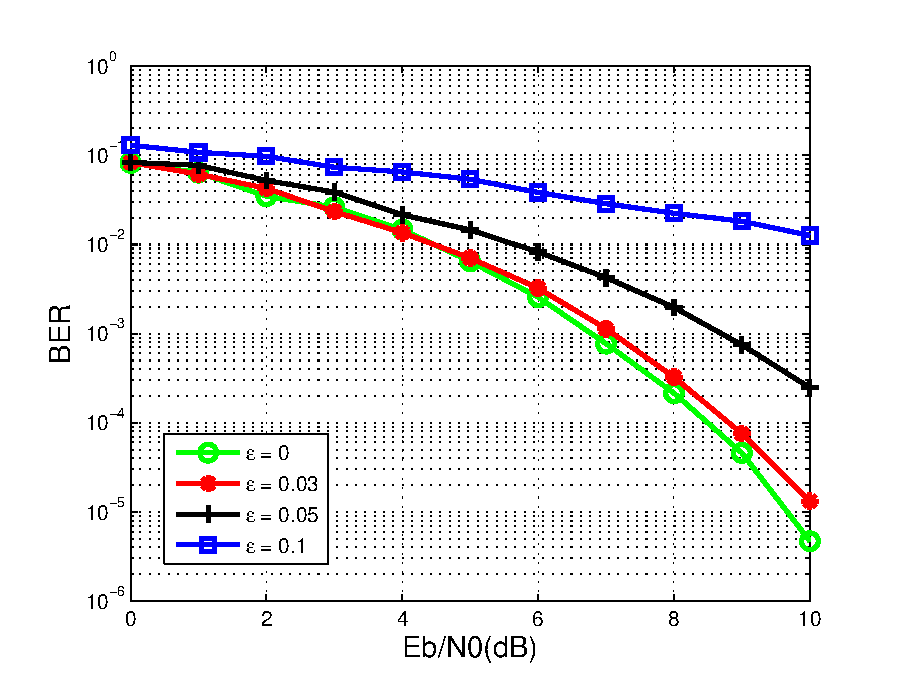
\includegraphics[width = 0.8\textwidth]{plot_ber_at_freq_error.eps}
\caption{有频偏下误比特率比较}\vspace{-1em}\label{plot_ber_at_freq_error}
\end{figure}
仿真数据采用~QPSK~调制。从图中可以看出,随着归一化频偏逐渐提高,变换域通信系统受到频偏的影响逐渐增大,性能逐渐降低。当归一化频偏达到~0.1~时系统性能已经严重下降。因此,在接收端频率同步就显得十分必要。


\subsection{基于循环前缀的同步算法}


我们知道,在~OFDM~技术中,为了消除码间干扰,对抗多径,传输信号使用了适当的循环前缀技术,只要循环前缀的长度~T~大于无线信道中的最大时延扩展,这样一个符号的多径分量就不会对下一个符号产生干扰,也不会因为多径的影响破坏子载波间的正交性。在混合载波通信系统中仍将采用分组传输的思想,利用循环前缀技术来对抗多径。根据最大似然原理的基本思想,可以利用发送信号结构中的循环前缀与信号本身的相关性来实现信号同步。

目前现有的基于循环前缀的比较经典的同步算法是文献[00599949]中提出的基于最大似然概率的同步算法,可将其应用在混合载波通信系统中。ML~算法对于定时和频偏的估计是以假设信道为加性高斯白噪声为前提的。这里给定~AWGN~信道下接收信号如下:
\begin{equation}
R(n) = T(n-\theta){e^{j2\pi \varepsilon k/N} } + z(n)
\end{equation}
~$\theta$~表示信号未确定的到达时间,$\varepsilon$~是归一化频偏。

ML~算法信号结构如图~\ref{ML_symbol_figure},
\begin{figure}[htbp]
\centering
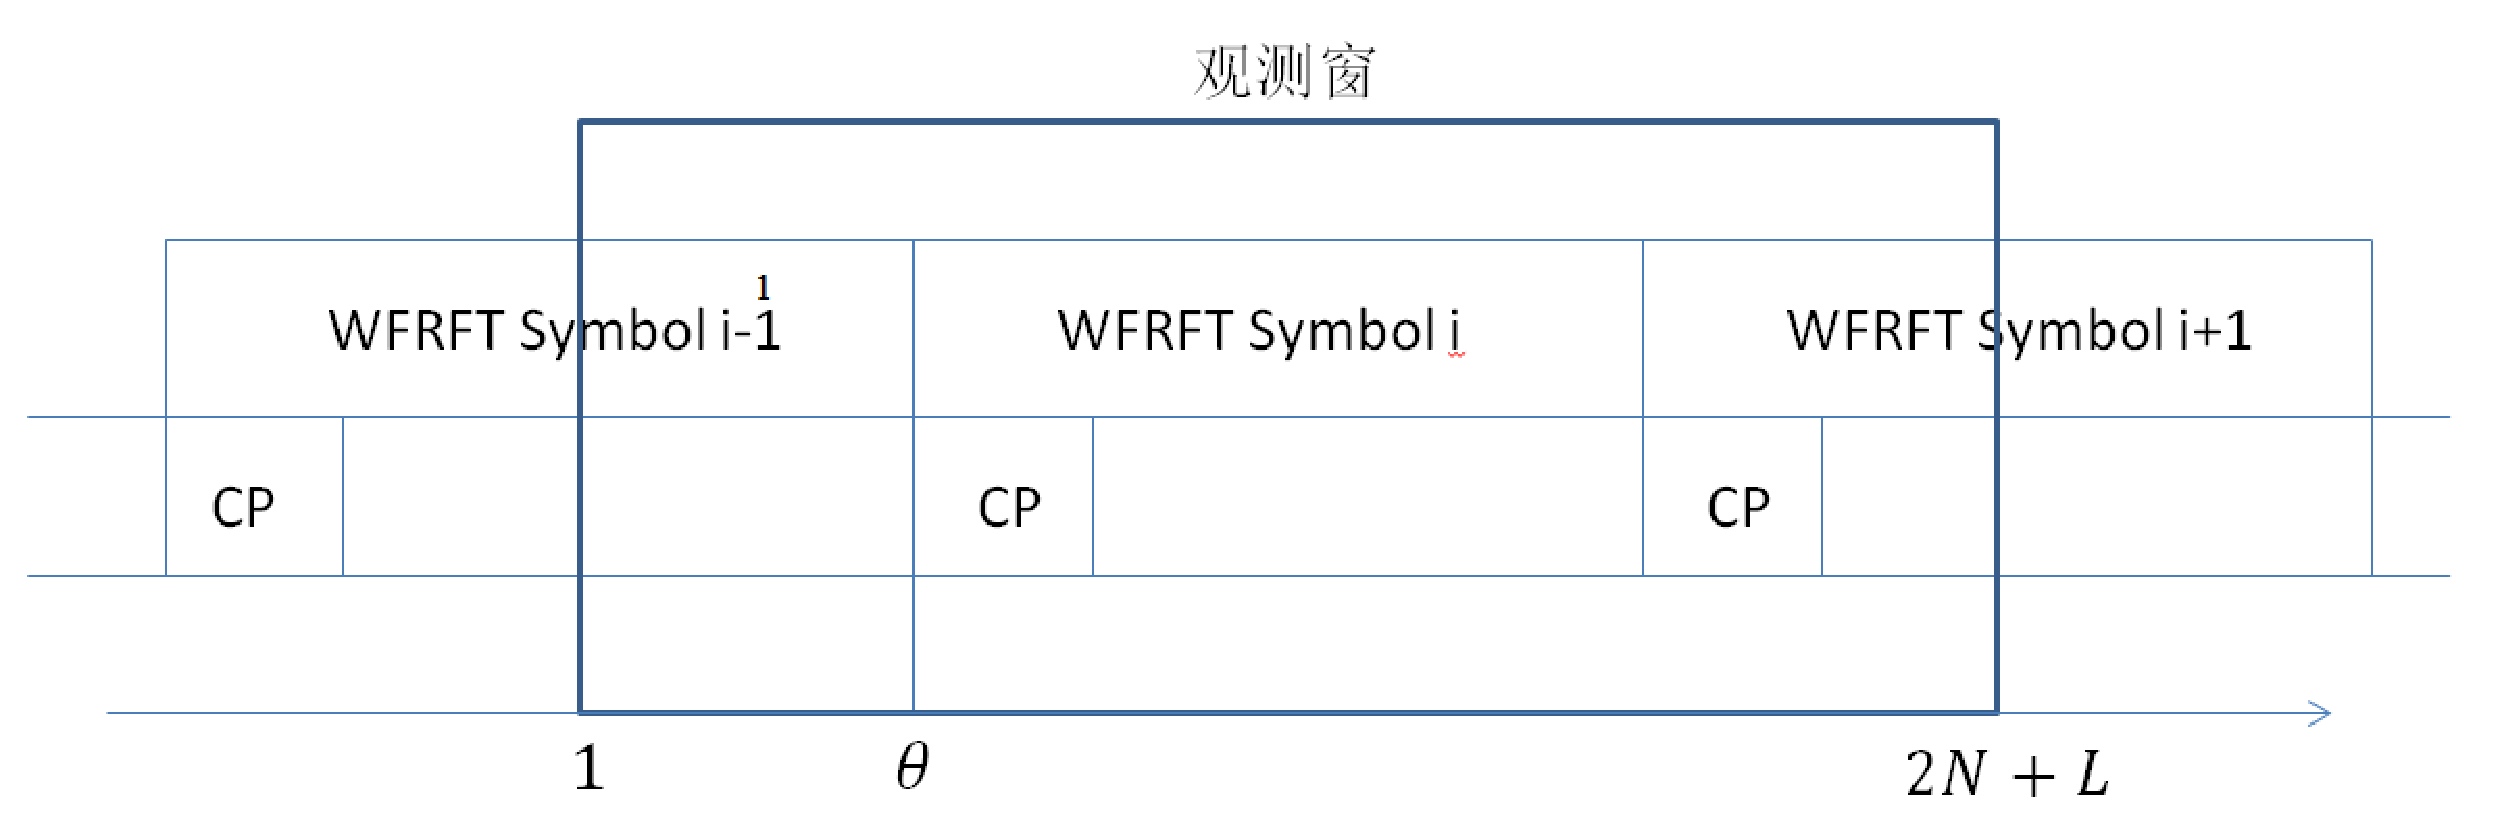
\includegraphics[width = 0.8\textwidth]{ML_symbol_figure.eps}
\caption{~ML~算法信号结构}\vspace{-1em}\label{ML_symbol_figure}
\end{figure}
假定一个~WFRFT~符号长度为~N,循环前缀长度为~L,我们将观测窗长度定为~$2N+L$,这样我们得到的采样点中包含一个完整的~WFRFT~符号(包含~$N+L$~采样点)。在这组采样点块中,符号的起始位置~$\theta$~对于接收端是未知的。观察窗口内接收信号的~$2N+L$~个采样值在给定同步参数定时误差~$\theta$~和频率偏移~$\varepsilon$~时的联合条件概率密度函数为:
\begin{equation}
\Lambda \left( {\theta ,\varepsilon } \right) = \log f\left( {r|\theta ,\varepsilon } \right)
\end{equation}
基于循环前缀同步的原理就是求使得~$\Lambda \left( {\theta ,\varepsilon } \right)$~最大时的定时误差和频率偏移。文献[]中对其进行化简推导得到
\begin{equation}
\Lambda \left( {\theta ,\varepsilon } \right) = \left| {\gamma \left( \theta  \right)} \right|\cos \left( {2\pi \varepsilon  + \angle \gamma \left( \theta  \right)} \right) - \rho \phi \left( \theta  \right)
\end{equation}
其中~$\angle$~为复数角度算子
\begin{equation}
\gamma \left( m \right) = \sum\limits_{k = m}^{m + L - 1} {r\left( k \right){r^*}\left( {k + N} \right)} ,
\end{equation}
\begin{equation}
\phi \left( m \right) = \frac{1}{2}\sum\limits_{k = m}^{m + L - 1} {{{\left| {r\left( k \right)} \right|}^2} + {{\left| {r\left( {k + N} \right)} \right|}^2}}
\end{equation}
\begin{equation}
\rho  = \left| {\frac{{E\left\{ {r\left( k \right){r^*}\left( {k + N} \right)} \right\}}}{{\sqrt {E\left\{ {{{\left| {r\left( k \right)} \right|}^2}} \right\}E\left\{ {{{\left| {r\left( {k + N} \right)} \right|}^2}} \right\}} }}} \right| = \frac{{\sigma _s^2}}{{\sigma _s^2 + \sigma _n^2}} = \frac{{SNR}}{{SNR + 1}}
\end{equation}

为了使最大似然函数能取得最大值,其中余弦项需为~1,似然函数变为
\begin{equation}
\Lambda \left( {\theta ,\varepsilon } \right) = \left| {\gamma \left( \theta  \right)} \right| - \rho \phi \left( \theta  \right)
\end{equation}
对~$\theta$~和~$\varepsilon$~的联合最大似然估计为
\begin{align}
&{\hat \theta _{ML}} = \arg \mathop {\max }\limits_\theta  \left\{ {\left| {\gamma \left( \theta  \right)} \right| - \rho \phi \left( \theta  \right)} \right\} \\
&{\hat \varepsilon _{ML}} =  - \frac{1}{{2\pi }}\angle \gamma \left( {{{\hat \theta }_{ML}}} \right)
\end{align}

图~\ref{ML_sim1}~给出~ML~算法的信号仿真,一个~WFRFT~符号长度选择1024点,循环前缀长度为128点,频率偏差为给定值~0.25,信噪比~$SNR=15dB$。
\begin{figure}[htbp]
\centering
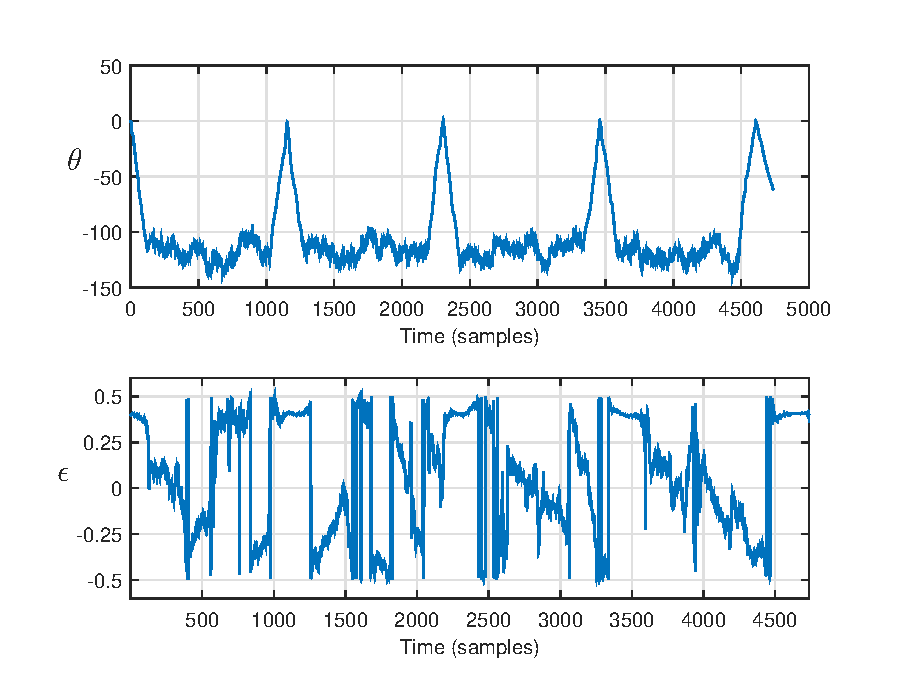
\includegraphics[width = 0.8\textwidth]{ML_sim1.eps}
\caption{~ML~算法信号仿真}\vspace{-1em}\label{ML_sim1}
\end{figure}
从图中可以看出,ML~算法的定时偏差估计曲线在正确的~CP~起始位置有着非常尖锐的峰值。仿真中存在~5~个~WFRFT~符号,所以有五个峰值,作为符号定时偏移的估计。其中横坐标为采样的点数,纵坐标为似然函数的值。在测度函数的最大值就是正确定时时刻。基于这一正确的符号定时点,又可以得出频偏的正确估
计值,如图。仿真时设定的频率偏移为0.25。可以看到,在正确的定时估计位置,对应的频率偏移都在0.25左右。

下面通过仿真分析~ML~算法的性能,性能指标为定时偏移和频率偏差估计的均方误差。首先参数估计的均方误差随偏差值大小的关系如图~\ref{Performance_by_freqError}~。
\begin{figure}[htbp]
\centering
\subfigure[频率估计性能]
{
\label{plot_freqMSE_freqError_at_diffSNR}
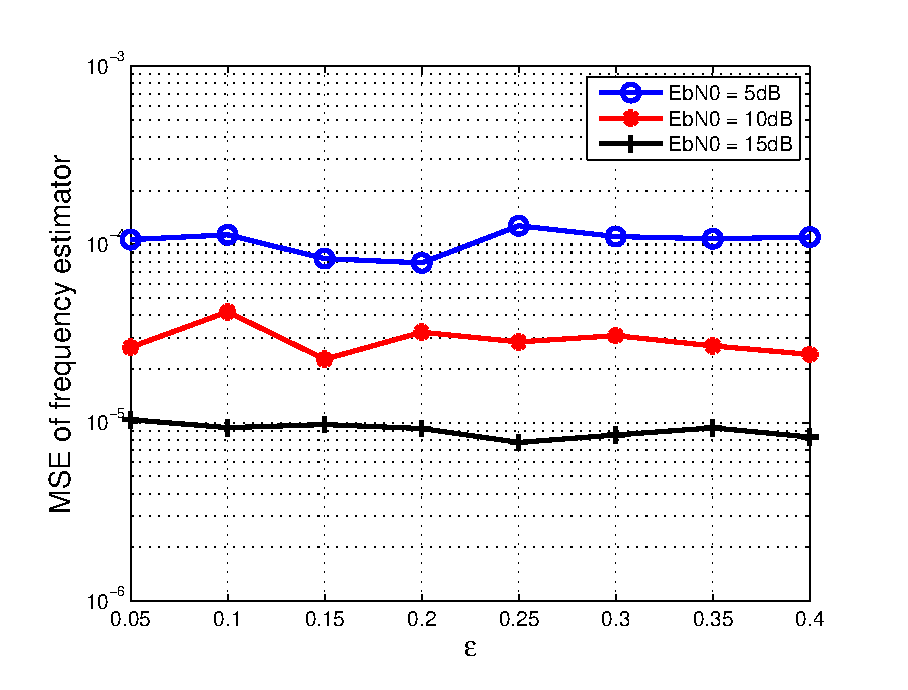
\includegraphics[width=0.4\textwidth]{plot_freqMSE_freqError_at_diffSNR.eps}
}
\subfigure[时间估计性能]
{
\label{plot_timeMSE_freqError_at_diffSNR}
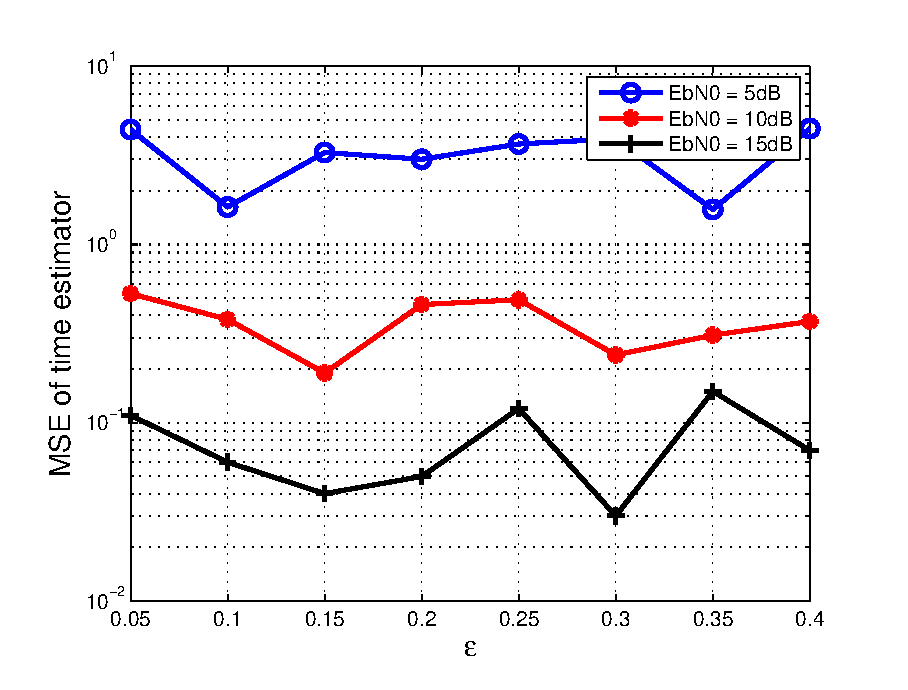
\includegraphics[width=0.4\textwidth]{plot_timeMSE_freqError_at_diffSNR.eps}
}
\caption{~ML~算法性能与频偏关系}\label{Performance_by_freqError}
\vspace{-1em}
\end{figure}
仿真条件为子载波数~2048~,循环前缀长度为~144。三条曲线信噪比分别取~5dB,10dB,15dB。归一化频偏值从~0.05~开始以~0.05~步进取到~0.4。首先显而易见的是信道条件越好,信噪比越大,估计的性能越好。还可以从图中看出无论频偏大小为多少,得到的频偏估计均方误差一定,即~ML~算法的频率偏移误差估计性能与频偏大小无关。

下面我们观察~ML~算法的估计性能都与哪些因素有关。图~\ref{Performance_by_alpha}~给出了不同阶数变换下算法的估计性能,仿真条件同样为子载波数~2048~,循环前缀长度为~144,归一化频率偏移为固定值~0.1。可以看出估计性能与混合载波通信系统的变换阶数无关。
\begin{figure}[htbp]
\centering
\subfigure[频率估计性能]
{
\label{plot_freqMSE_alpha_at_diffSNR}
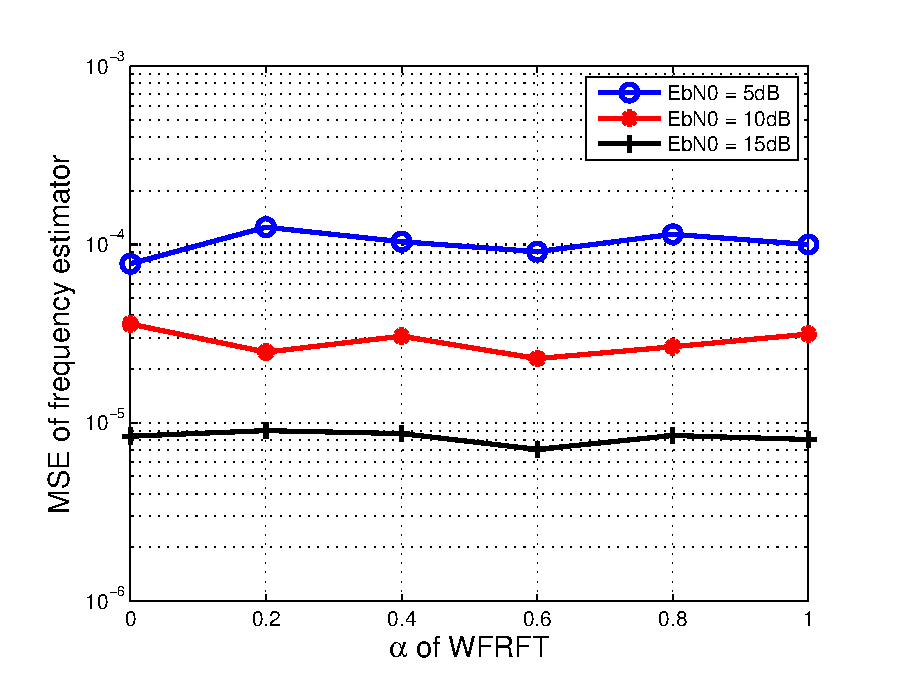
\includegraphics[width=0.4\textwidth]{plot_freqMSE_alpha_at_diffSNR.eps}
}
\subfigure[时间估计性能]
{
\label{plot_timeMSE_alpha_at_diffSNR}
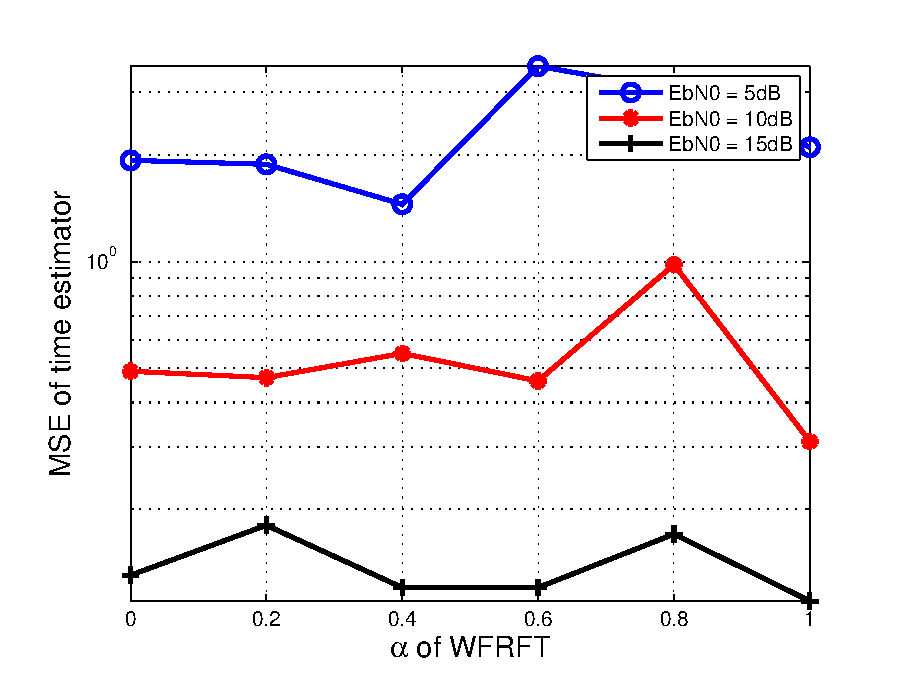
\includegraphics[width=0.4\textwidth]{plot_timeMSE_alpha_at_diffSNR.eps}
}
\caption{~ML~算法性能与变换阶数关系}\label{Performance_by_alpha}
\vspace{-1em}
\end{figure}

图~\ref{Performance_by_CP}~给出了不同循环前缀长度下定时估计和频偏估计的均方误差随循信噪比的变换关系。
\begin{figure}[htbp]
\centering
\subfigure[频率估计性能]
{
\label{plot_freqMSE_EbN0_at_diffCP}
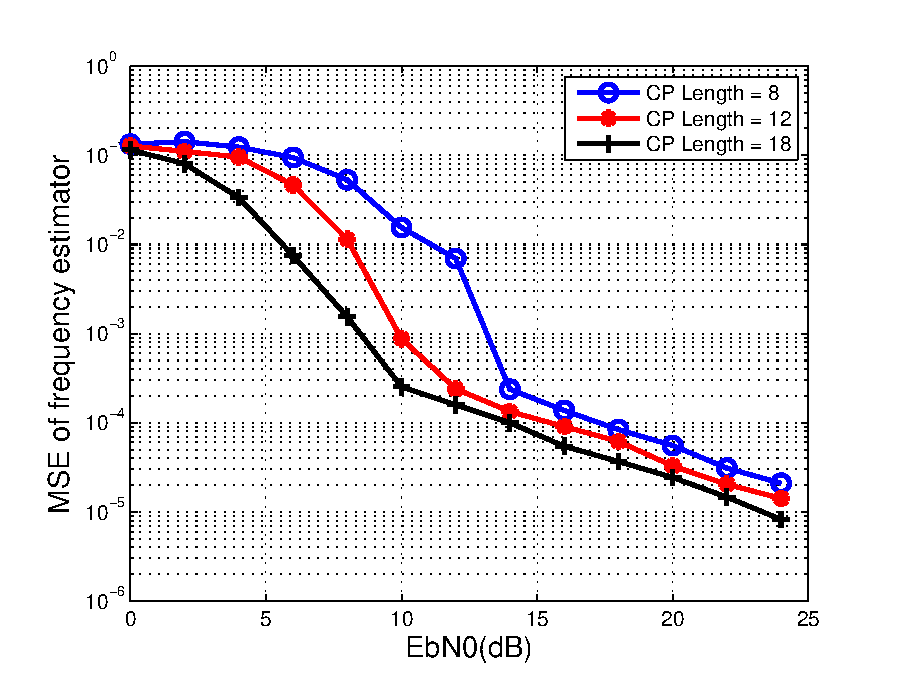
\includegraphics[width=0.4\textwidth]{plot_freqMSE_EbN0_at_diffCP.eps}
}
\subfigure[时间估计性能]
{
\label{plot_timeMSE_EbN0_at_diffCP}
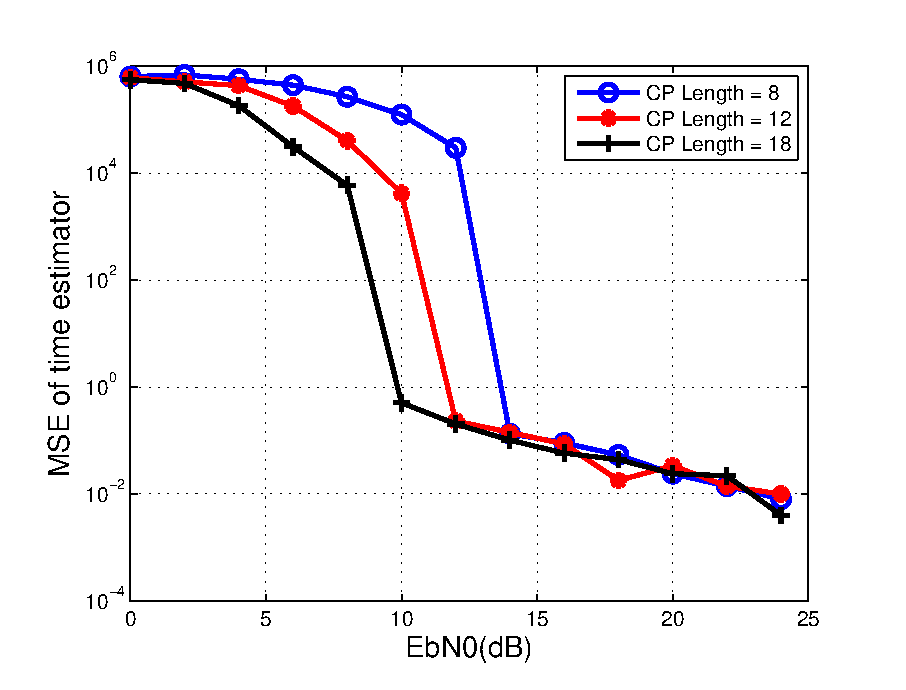
\includegraphics[width=0.4\textwidth]{plot_timeMSE_EbN0_at_diffCP.eps}
}
\caption{~ML~算法性能与循环前缀长度关系}\label{Performance_by_CP}
\vspace{-1em}
\end{figure}
仿真条件为子载波数~2048~,分别去循环长度为~8,12,18。归一化频偏设定为~0.25。可以看出,在同一信噪比条件下,频偏估计均方误差随着循环前缀的增加而下降,当超过一定门限(约12dB)时,均方误差随着信噪比的下降趋势会便缓慢,但是同定时估计性能相比下降的更为明显。在门限之前,循环前缀越长,同一信噪比下所对应的频率同步均方误差越小,而超过此特定门限之后,增加循环前缀所带来的性能优势仍然存在但变得不再明显。而定时估计性能同样存在一个门限(约12dB),在随信噪比的增加通过门限时不同长度循环前缀的定时估计均方误差迅速下降,趋于重合,说明超过门限之后不同循环前缀长度的定时同步性能已经基本相同。

从最大似然函数的表达式不难看出,每计算一个采样点的计算量较大,在实际实现过程中比较困难。为了解决这个问题,压缩同步算法的运算量,文献提出了最大相关(MC)算法,它仅是~ML~算法的简化算法,只考虑了~CP~与数据部分的相关性,计算复杂度大大降低。
MC~算法的最大似然函数为:
\begin{equation}
\Lambda \left( {\theta ,\varepsilon } \right) = {\left| {\gamma \left( \theta  \right)} \right|^2} = {\left| {\sum\limits_{n = \theta }^{\theta  + L - 1} {r\left( n \right){r^*}\left( {n + N} \right)} } \right|^2}
\end{equation}

因而得到的联合估计为:
\begin{align}
&{{\hat \theta }_{MC}} = \arg \mathop {\max }\limits_\theta  \left\{ {{{\left| {\gamma \left( \theta  \right)} \right|}^2}} \right\} \\
&{{\hat \varepsilon }_{MC}} =  - \frac{1}{{2\pi }}\angle \gamma \left( {{{\hat \theta }_{MC}}} \right)
\end{align}
下面给出~MC~算法的运算框图~\ref{MC_kuangtu}~。
\begin{figure}[htbp]
\centering
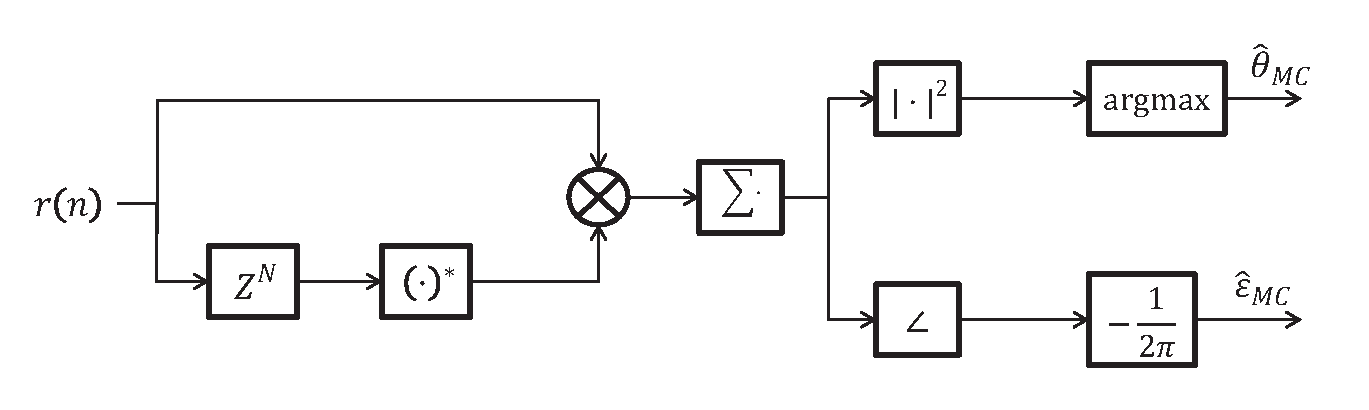
\includegraphics[width = 0.8\textwidth]{MC_kuangtu.eps}
\caption{~MC~算法框图}\vspace{-1em}\label{MC_kuangtu}
\end{figure}

可以看到运算复杂性大大降低,实际上从最大似然函数的表达式也能看出,ML~中的能量项被忽略,仅保留相关函数项,这对于频偏估计是没有影响的,但牺牲了定时估计的准确性。

综上所述,ML~算法应用在HC通信系统中,有着不占用额外频谱资源,同时计算量小的优点。但同时极易受到干扰,包括信道,滤波等等,都在一定程度上破坏CP前后一致性,可以通过联合多个符号CP同时,进行辅助同步,显著降低误差,虽然并未额外浪费频谱资源,但由于联合多个符号进行,会增加接收端信号处理延时。而在实际应用中,当存在多径干扰时,CP部分会与数据部分的相关性受到影响,此时的估计抖动较大,因为~ML~算法本事是以~AWGN~信道为前提而进行的,而无线通信中的信号基本都会受到严重的多径干扰,故如何有效抗多径干扰是此同步算法急需解决的问题。






% !Mode:: "TeX:UTF-8"

\section{研究方案及进度安排,预期达到的目标和取得的研究成果}
\subsection{研究方案}
研究目标为设计一种适用与混合载波通信系统的同步方案,包括最佳采样时刻同步、时域同步和载波频率同步。比较的标准为同步概率和同步参数估计的均方误差(MSE)。同步方式计划采用基于辅助序列的同步方法,首先设计同步序列结构,比如采用~CAZAC~序列及其共轭,然后设计接收端定时度量函数,使得定时函数在同步位置保持尖锐,即得到较好同步效果的,然后根据序列结构设计频偏度量函数,估计出时域偏差与频率偏差,完成同步过程。

研究过程大致分为三步。

第一步大量查阅文献,进行同步算法的总结综述,对不同算法进行理论分析和比较,明确适用范围以及优缺点。

第二步探索现有同步算法与混合载波通信系统的兼容性,选取适用于混合载波通信系统的同步算法,并尝试应用在混合载波通信系统中,通过仿真来进行性能分析,比较各实现方法的计算复杂度、同步速度、同步参数估计的均方误差。

第三步设计适用于混合载波通信系统的新型同步序列结构,设计在同步时刻更加尖锐的定时度量函数,给出混合载波通信系统的同步方案。

\subsection{预期达到的目标和取得的研究成果}
完成混合载波通信系统同步方案的设计与性能仿真,从而更加完善基于~WFRFT~混合载波通信系统的研究。

\subsection{进度安排}
\begin{table}[htbp]
\centering
\caption{进度安排}\label{table3}\vspace{-0.5em}\zihao{5}
\begin{tabularx}{0.8\textwidth}{lX}
\toprule
2017.6~2017.8 & 查阅先关文献,确定课题内容及方案。\\
2017.8-2017.10 & 完成5.1节中第一步,对现有同步算法进行综述与分析。\\
2017.10-2017.12	& 完成5.1节中第二步,探索分析现有同步算法,以及应用在混合载波通信系统的可能性,并将适用的算法尝试应用在混合载波通信系统中。\\
2017.12-2018.2 & 继续5.1节中第二步,对应用于混合载波通信系统的同步算法进行进行仿真对比分析。\\
2018.2-2018.5 & 完成5.1节中第三步,设计混合载波通信系统同步解决方案,并进行可行性分析与性能仿真。\\
2018.5-2018.7 & 撰写毕业论文,准备答辩。\\
\bottomrule
\end{tabularx}
\end{table}


\section{为完成课题已具备和所需的条件和经费}
近年来关于混合载波通信系统的研究比较多,可提供研究思路的参考的文献很容易获取。基本理论比较成熟也为本项研究奠定了一定的理论基础。本课题来源于国家重点基础研究发展计划(973计划)——异构网络协同信号处理理论与方法,项目正顺利进行,且已经有了一些成果与经验,也会为本课题研究的开展提供有力的支撑。为完成本课题,还需要查阅大量文献资料,并且可能需要借阅或者购买一些参考书籍。本课题所需的研究经费和实验设备条件已具备。


\section{预计研究过程中可能遇到的困难和问题,以及解决的措施}
本课题中基于混合载波通信系统的同步方案设计还是比较新颖的,所以研究中同步偏差对通信系统的影响,以及各种同步算法的原理与同步定时函数的设计会使用较多的数学方面的知识。因而数学理论的学习以及公式的推导可能需要大量的时间。在研究的过程中,需要查阅相关文献,并及时与老师及实验室师兄、师姐们沟通。


\bibliographystyle{GBT7714-2005NLang-HIT}
\addtolength{\bibsep}{-0.8em}
\nocite{*}
\bibliography{reference}

\end{document}
